\documentclass[14pt,a4paper]{memoir}
\usepackage{listings}
\usepackage[framemethod=tikz]{mdframed}
\usepackage{graphicx}
\usepackage{float}
\usepackage{xcolor}
\usepackage{textcomp}
\usepackage{menukeys}
\usepackage{gensymb}
\usepackage{amsmath}
\usepackage{hyperref}
\graphicspath{ {./images/} }
\usepackage{xepersian}
\settextfont{XB Zar}
\setlatintextfont{Times New Roman}
\deflatinfont\mono[Scale=.7]{Courier New}




\definecolor{mycolor}{rgb}{0.122, 0.435, 0.698}

\newmdenv[innerlinewidth=0.5pt, roundcorner=4pt,linecolor=mycolor,innerleftmargin=6pt,
innerrightmargin=6pt,innertopmargin=6pt,innerbottommargin=6pt]{mybox}


\newmdenv[innerlinewidth=0.5pt, roundcorner=4pt,linecolor=mycolor,innerleftmargin=6pt,
innerrightmargin=6pt,innertopmargin=6pt,innerbottommargin=6pt, backgroundcolor=yellow]{tip}




\begin{document}
		
		
		
\frontmatter
	
	\title{ بازی سازی و برنامه نویسی خلاقانه پایه}
	\author{چوبک بیدپا}
	\date{}
	\clearpage\maketitle
	\thispagestyle{empty}
	
\includegraphics[scale=0.6]{Cover}	
	\newpage
	
		

	
	\begin{mybox}
		\begin{center} عرضه شده تحت لیسانس MIT\\ 1397
				\vfill
				نویسنده: چوبک بیدپا
				\vfill
				سال عرضه: 1397
				\vfill
				کاملا رایگان \vfill
				جهت برقراری ارتباط با چوبک بیدپا از ایمیل \url{chubakbidpaa@riseup.net} استفاده نمایید.
	\end{center}	


	\end{mybox}
 
 
	 \vfill
	 
	 به خاطر اینکه بخش قابل توجهی ازین کتاب، از آموزشهایی که تحت لیسانس \lr{Creative Commons}، MIT و GPL عرضه شده اند استفاده میکند، استفاده ، تکثیر و آموزش این کتاب، به شرط نام بردن نویسنده یعنی شخص حقیقیِ چوبک بیدپا، آزاد میباشد.
	 
	 توجه داشته باشید که فایلهایی که همراه کتاب به فروش گذاشته شده اند، غیرقابل تکثیر بوده، و آپلود آنها توسط شخص حقیق چوبک بیدپا قابل قبول میباشد.
	 
	 تحت قوانین Transference، شما جهت استفاده از بخشهای این کتاب که توسط افراد دیگر نگاشته شده اند احتیاجی به اجازه از آنها ندارید.
	 
	 در آخر، قابل توجه باشد که این کتاب یک پروژه ی اشتیاقی \footnote{\lr{Passion Project}} می باشد، و نه پروژه ای که برای به دست آوردن پول نوشته شده است. برای همین، مرام را به جای آورید و آنرا در جای دیگر آپلود نکنید.
	 
	 لطفا فایلهایی که همراه کتاب خریده اید نیز جایی کپی نکنید. قیمت فایلها با توجه به استطاعت خوانندگان، با الگوریتمی پیچیده\footnote{با بیشتر شدن تعداد خریدارها، قیمت کاهش میابد.} تعیین شده است. برای همین همه میتوانند آن را بخرند. آپلود فایلهای کتاب در جای دیگر، پایرسی حساب میشود و از لحاظ اخلاقی، کاریست نپسندیده.
	 
	 اما تکثیر خود کتاب با ذکر منبع آزاد است.
	  
	 \textbf{نکته:} کدهای کتاب در فایل خریداری شده حی و حاظر آماده ی کپی میباشد.
	 
	 
	 
	 \chapter*{قراردادهای کتاب}
	 
	 \begin{enumerate}
	 	\item  بخشهای کتاب: این کتاب به دو بخش برنامه نویسی خلاقانه\footnote{\lr{Creative Programming}}، و بازی سازی تقسیم شده است.
	 	\item  نکته: نکته های خاص کتاب در به این صورت مشخص شده اند:
	 		
	 	
	 				\begin{tip}
	 					نکته اینجاست که....
	 				\end{tip}
	 
	 \item استفاده از فایلها: اگر فایلی لازم باشد، نام و آدرس آن در فایل زیپ دانلود شده نوشته خواهد شد.
	 \item یو آر الها به صورت \url{https://google.com} نوشته خواهند شد.
	 \item متن پررنگ: وقتی لازم است روی کلمه ای تاکید کنم، یا کلمه جدید است و قبلا استفاده نشده، از \textbf{متن پررنگ} استفاده خواهم کرد.
	 \item  دکمه ها به صورت آیکون تعریف شده اند. یادتان باشد که دکمه ی \keys{\shift} نشانگر دکمه ی شیفت میباشد. دکمه ی بالا \keys{$\uparrow$} میباشد.
	 \item کد: کدهایی لازمه به صورت زیر نوشته خواهند شد.
	 
	 
	\begin{latin}
	\mono{	\begin{lstlisting}
for i:=maxint to 0 do
begin
{ do nothing }
end;
Write('Case insensitive ');
Write('Pascal keywords.');
		\end{lstlisting}}
	
	\end{latin}
	 
	\end{enumerate}
	 
	 
	 \tableofcontents
	 \mainmatter
	 
	 \chapter{چند کلمه با خواننده} \label{foreword}

	«آزادی خود را گرامی بدارید، وگرنه آنرا از دست میدهید.»
	امروزه، جبهه های مختلفی هستند که بر آزادی اطلاعات عقیده دارند. یکی از آنها نهاد گنو\footnote{GNU} است که کِرنل سیستم عامل لینِکس\footnote{Linux} را در دست دارد. دیگری مازیلاست\footnote{Mozilla}، که مرورگر فایرفاکس\footnote{Firefox} را منتشر کرده است. 
	
	من به شخصه معتقدم آژادی اطلاعات از آزادی بیان مهمتر است، چون اگر اطلاعات را برای خود نگه داریم، کمتر کسی راههای اشاعه ی آزادی بیان را یاد خواهد گرفت، یا اصلا خواهد دانست که آژادی بیان چه هست. 
	
	این کتاب نه تنها بر پایه ی عقیده به آزادی اطلاعات\footnote{\lr{Freedom of Information}} مجانی است، بلکه یکی از دلایل مجانی بودن آن اینست که تمام آن مال من نیست، بلکه، حدود 30\% این کتاب، ترجمه ی آموزشهای اینترنت، با اجازه از صاحبان آنهاست. 20\% این کتاب، از داکیومنتشنهای رسمی برداشته شده  و 50 درصد باقی را خودم نوشته ام.
	
	شاید برایتان سوال باشد چرا این کتاب را نگاشت کرده ام. دلیل اصلی آن اینست که دلیلی داشته باشم تا برنامه نویسی را ادامه دهم. بعضی ها پروژه مینویسند، بعضی ها کتاب مینویسند. من در لفافه ی کتاب، پروژه مینوسم. تمام پروژه های کتاب اریجینال بوده، و فایلهایی که همراه کتاب خریده اید، کار من هستند.
	
	دلیل دیگری که این کتاب را نوشته ام، اینست که کتاب های بازی سازی به زبان فارسی کم هستند، و کمتر کسی در ایران از برنامه نویسی خلاقانه خبر دارد. سعی من درینست که با نوشتن در مورد این دو دیسیپلین دوست داشتنی، فرهنگ آنها را در کشور اشاعه بدهم.
	
	از سابقه ام در برنامه نویسی و بازی سازی بگویم. من از شانزده سالگی\footnote{الان بیست و پنج ساله ام.} کم و بیش در برنامه نویسی، و گهگاهی ساخت بازی، فعال بوده ام. مانند خیلی ها از نرم افزار \lr{Game Maker} کارم را شروع کردم و با آن چندین بازی مانند تتریس، بریک اوت و... ساختم. من چندین بازی تحت اسکی مانند بلک جک نیز نوشته ام. من زبانهای \lr{C++}، پایتان، و C را میدانم و با زبان اسکریپت نویسی چندین نرم افزار آشنایی دارم. به علوم نرم مانند ادبیات انگلیسی آشنایی آکادمیک دارم و در حال حاظر دانشجوی برنامه نویسی ام.
	
	سابقه ی من در برنامه نویسی خلاقانه کمتر است. دو سال پیش بود که با نرم افزار افتر افکتس\footnote{\lr{After Effects}} آشنا شدم و به صرافت نوشتن پلاگین برایش افتادم، و طی این امر، با کتابخانه ی Cinder برای \lr{C++} آشنا شدم. و از آنجا بود که با زبان Processing و شیدر ها آشنا گردیدم. الان تسلط کافی برای آموزش پایه ی شیدرها و زبانها و کتابخانه های برنامه نویسی خلاقانه دارم.
	
	بگذارید در مورد چارچوب کتاب کمی صحبت کنم. در این کتاب، دو بخش داریم، برنامه نویسی خلاقانه، و بازی سازی که به دو بخش Asset و برنامه نویسی تقسیم میشود. در بخش اَسِت سعی شده با استفاده از برنامه های مختلف، ساخت اسپرایت، تایل، اسپرایت شیت، تایل شیت، عکس پس زمینه، مدل سازی سه بعدی، و تکسچر و متریال  را آموزش دهم. در بخش برنامه نویسی کتابخانه ی Arcade پایتان، کتابخانه ی SFML سی پلاس پلاس، و انجین Godot\footnote{تلفظ این انجین، گَدو میباشد.} آموزش داده خواهد شد. اگر قرصت شد، آموزشی کوتاه برای ساخت انجین خودتان را خواهم نوشت.
	
	قبل از هرچیزی دو چیز باید یادآوری شود: برنامه نویسی، و ریاضی. من زیاد در مورد این دو کانسپت حرف نمیزنم، چون وظیفه ی خود خواننده است که این دو را از قبل یاد داشته باشد، اما فقط در حد یادآوری، در مورد این دو حرف خواهم زد.
	 
		 در آخر، در این دنیای پر هیر و گیر، اگر عشقی\footnote{Passion} به چیزی دارید که به شما آرامش میدهد، نیکوست. و اگر این کتاب برای پیدا کردن این عشق کمک میکند، خوشحالم.
	 
	 \begin{flushleft}
	 	چوبک بیدپا
	 	مشهد - 1397
	 \end{flushleft}
	 
	 
	 
	 \chapter{نگاهی کوتاه به ریاضی لازمه}\label{math}
	 \section{توابع}\label{functions}

یک تابع\textbf{\footnote{Function} به صورت زیر نشان داده میشود:
\[y = f(x)\]}

وظیفه ی یک تابع، تغییر عدد داده شده بر اساس قوانین داده شده است. به این قانون، تابع میگویید. مثلا تابع \(f(x) = x^2\) که به آن تابع مربع می گویند، وظیفه اش بردن عدد به توان دو است. به عکس تابع، تابع \textbf{معکوس}\footnote{Inverse} میگویند و به صورت زیر نشان داده میشود:

\[y = f^{-1(x)}\]

مثلا معکوس تابع مربع، تابع ریشه دو یعنی $ f(x) = \sqrt{x} $ میباشد. میتوان دو تابع را با هم به صورت $ f(g(x)) $ ترکیب کرد که به آن تابع مرکب میگویند. از دیگر عملیاتها عبارت است از:

\[  (f + g)(x) = f(x) + g(x) \]
\[ (f - g)(x) = t f(x) - g(x) \]
\[  (f * g)(x) =  f(x) * g(x) \]
\[  \left(\frac{f}{g}\right)(x) =  \frac{f(x)}{g(x)} \]

به تمام اعدادی که تابع میپذیرد، \textbf{دامنه}\footnote{Domain}، و تمام اعدادی که تابع خارج میکند، \textbf{برد}\footnote{Range} خوانده میشود. دامنه ی یک تابع را ما تعیین میکنیم، اما برد آن را خود تابع تعیین میکند.

در آخر، بگذارید بگویم که تابع مانند یک ماشین است. ورودی آن $ x $ و خروجی آن $ f(x) $ است. در برنامه نویسی از توابع استفاده ی زیادی میشود. در بخش برنامه نویسی خواهید خواند.

\section{بردارها}\label{vector}

اگر فضای دوبعدی را به دو بخش نقاط افقی و نقاط عمودی تقسییم کنیم، \textbf{بردار}\footnote{Vector} خطی است که چهار نقطه را به هم وصل میکند.

\includegraphics*[scale=0.3]{Vector} 

بردار را به صورت زیر نشان میدهند:

\[ \vec{V} = (x_1, y_1) + (x_2, y_2) \]
	 
	 صفحه ی مختصات را به این صورت میکشیم: \vfill
	 \begin{center}
	 	\includegraphics*[scale = 1]{coordinate_system}
	 \end{center}
	 
	 که به آن \textbf{دستگاه مختصات دکارتی}\footnote{\lr{Carthesian Coordinate System}} میگویند. در دستگاه مختصات دکارتی، دو محور $ X $ و $ Y $ به ترتیب محور افقی و عمودی ما را تشکیل می دهند. ما مختصات یک نقطه را در پرانتز به صورت $ (X, Y) $ نشان میدهیم. همانطور که گفته شد، خطی که دو نقطه را به هم وط کند، بردار نام دارد.
	 
	 در جبر خطی، بردار  به صورت:	 
	 \[\vec{V} = \begin{pmatrix}
	 X \\ Y
	 \end{pmatrix}
	 \] 	 
	 نشان داده میشود و نقطه ی اول آن، مسقط الرأس دستگاه مختصات یعنی $ (0, 0) $ میباشد. 	 
\begin{figure}[H]
	\centering
		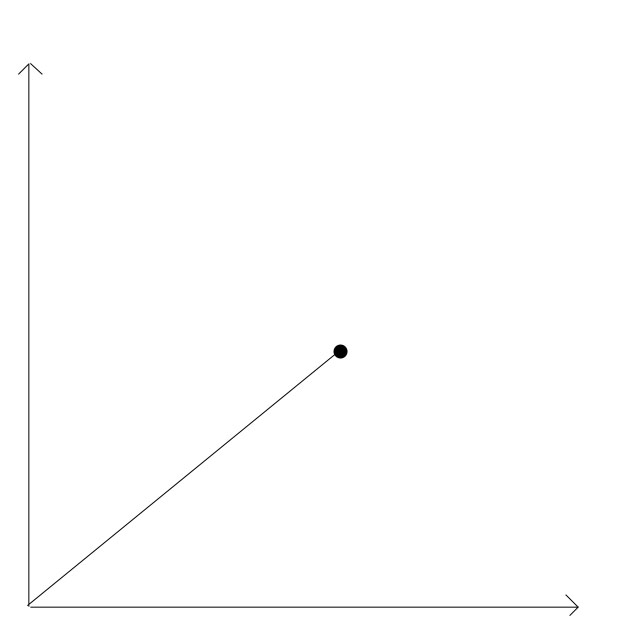
\includegraphics[scale=0.8]{LinAlgVec}
	
\end{figure}
		به برداری که مختصات افقی، یا عمودی آن، یک باشد بردار واحد میگویند. بردار واحد افقی را $ \vec{i} $ و بردار افقی عمودی را $ \vec{j} $ میگویند. بردار ها را میتوان به صورت مضربی از بردار واحد نشان داد مثلا بردار $ \vec{V} = \begin{pmatrix}
	X \\ Y
	\end{pmatrix}$ را میتوان به صورت $ X\vec{i} + Y\vec{j} $ نشان داد. 
	
	
	
	
یک بردار دارای دو خصیصه می باشد. \textbf{جهت}\footnote{Direction} و \textbf{مقدار}\footnote{Magnitude}. که به صورت زیر نشان داده میشود:

	
		 \begin{center}
		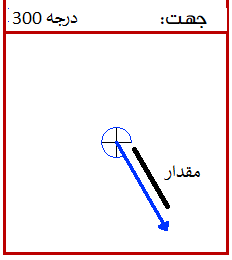
\includegraphics[scale=1]{DirMag}
	\end{center}

برای به دست آوردن مقدار بردار ازین فرمول استفاده میکنیم:
\[ |\vec{V}| =  \sqrt{x^2 + y^2} \]
	
	
	
	 
	 دو بردار را میتوان به صورت زیر جمع کرد:
	 
	 
	 	 \begin{center}
	 	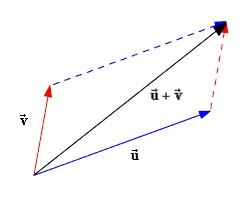
\includegraphics[scale=1]{VectorAdd}
	 \end{center}
 
 و به این صورت تفریق کرد:
  
 \begin{center}
 	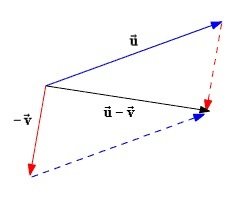
\includegraphics[scale=1]{VectorSubtract}
 \end{center}
 
	 
	 
	 اما دو نوع ضرب برداری داریم. \textbf{ضرب تقطه ای}\footnote{\lr{Dot Product}} و \textbf{ضرب صلیبی}\footnote{\lr{Cross Product}}. قبل ازین که پیش بروید، قسمت مثلثات \(\ref{trig}\) را بخوانید. فرض کنید دو بردار به صورت زیر هستند:
	 
	 
	  \begin{center}
	 	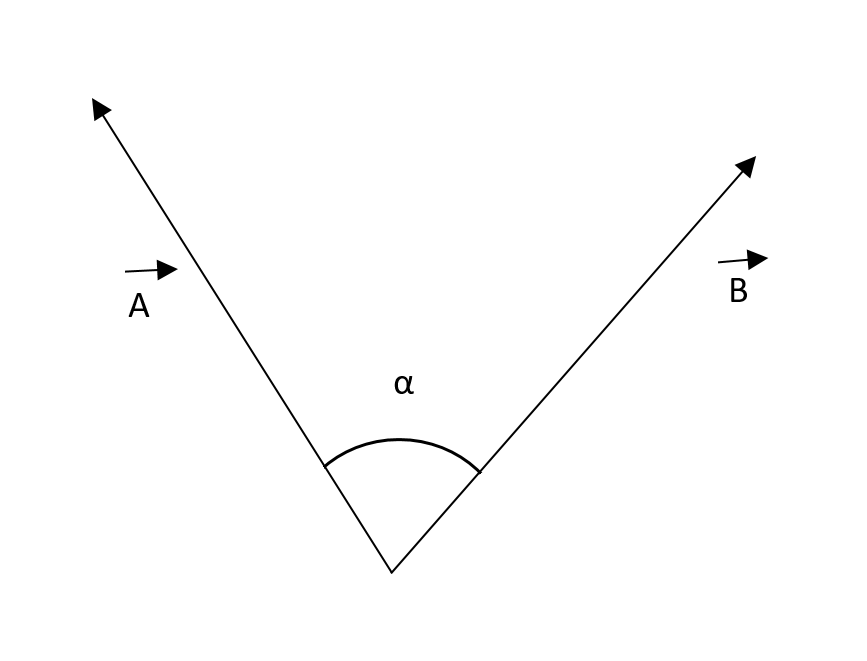
\includegraphics[scale=0.3]{Product}
	 \end{center}
	 
	 
	 ضرب نقطه ای به صورت زیر تعریف میشود:
	 
	 \[ \vec{A}.\vec{B} = |A||B|\cos \alpha \]
	 
	 و ضرب صلیبی ازین فرمول استفاده میکنیم.
	 \[ \vec{A} \times \vec{B} = |A||B|\sin \alpha \vec{n} \]
	 
	 
	 که  $\vec{n} $ برداری \textbf{پایه}\footnote{\lr{Basis Vector}}  عمود بر دو بردار است. برای به دست آوردن $\vec{n}$ کافیست از انگستان وسط، اشاره، و شصت خود استفاده کنید. انگشت شصت شما، همواره بردار واحد عمود است، که مضربی از ضرب صلیبی دو بردار می باشد.
	 
	 
	 \section{مثلثات}\label{trig}
	 
	 مثلثات بحثیست پیپیده. و من نیز ریاضیدان نیستم پس به کمی در مورد این مبجث قناعت میکنیم.  قبل از هرچیزی، بگذارید در مورد \textbf{دستگاه مختصات قطبی}\footnote{\lr{Polar Coordinate System}} حرف بزنم. دستگاه مختصات قطبی، مانند دستگاه مختصات دکارتی، دارای دو محور عمودی و افقی است. اما در این دستگاه مختصات، ما یک نقطه را، عوض $ X $ و $ Y $ توسط یک زاویه $ \alpha $ و یک بردار شعاع $ \vec{r} $ نشان میدهیم:
	 
	 
	 
	 	  \begin{center}
	 	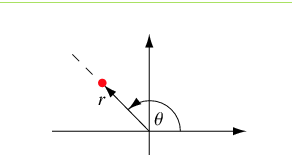
\includegraphics[scale=1]{Polar}
	 \end{center}
 
 در برنامه نویسی خلاقانه، دستگاه مختصات قطبی کاربردهای زیادی دارد. اما در کامپیوتر، \textbf{پیکسلها}\footnote{در مورد پیکسلها به وفور حرف خواهم زد.} در دستگاه مختصات دکارتی قرار دارند. حلال مشکلات ما، مثلثات است.
 یک دایره ی واحد را در دستگاه مختصات  قطبی کنید که شعاعش 1 میباشد:
  \begin{center}
 	\includegraphics[scale=1]{UnitCIrcle}
 \end{center}

اگر زاویه ی $   30\degree   $ را انتخاب کرده و یک مثلث قائم الزاویه دور آن بکشیم:


	   \begin{center}
	 	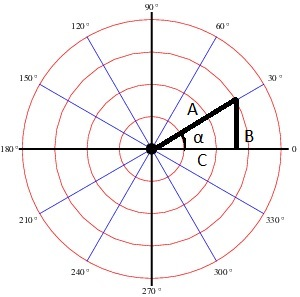
\includegraphics[scale=1]{ThirtyDegrees}
	 \end{center}
	 
	 سینوس و کسینوس زاویه 30 درجه که اینجا $ \alpha $ نامیده میشود، به صورت زیر تعریف میگردد:
	 \[ \sin \alpha = \frac{\text{مقابل}}{\text{وتر}} \]
	 
	 و:
	 
	 \[ \cos \alpha = \frac{\text{مجاور}}{\text{وتر}} \]
	 
	 همچنین تانژانت و کتانژانت به صورت زیر تعریف میشوند:
	 
	  \[ \tan \alpha = \frac{\sin \alpha}{\cos \alpha} \]
	  
	  
	  و 
	  \[ \cot \alpha = \frac{\cos \alpha}{\sin \alpha} \]
	  
	  
	  درجه، تنها واحد اندازه گیری زاویه نیست. واحد دیگر، \textbf{رادیان}\footnote{Radians} نام دارد. یک زاویه در رادیان، بین $ 0 $ و$   2\Pi $ قرار دارد. ارزش $ \Pi $ حدود $ 3.1415926535 $ است. ما برای کار با پیکسلها، ارقام اعشار بیشتر ازین نیز نیازمندیم. برای تبدیل درجه به رادیان:
	  \[ n\degree \times 	  \frac{\pi}{180} \]
	  
	  , و بالعکس:
	  
	  \[ n \space \textrm{rad} \times 	  \frac{180}{\pi} \]
	  
	  
	  
	  
	  توابع مثلثاتی توسط \textbf{هویتهای مثلثاتی}\footnote{\lr{Trigonometric Identities}} به هم ربط داده میشوند. بعضی ازین هویتها عبارتند از:
	  
	  \[ \sin^2 \alpha + \cos^2 \alpha = 1 \]
	  \[ \sin(-\alpha) = -\sin\alpha \]
	  \[ \cos(-\alpha) = \cos(\alpha) \]
	  \[ \sin(\alpha\pm\beta) = \sin\alpha\cos\beta \pm\cos\alpha sin\beta \]
	  \[ \cos(\alpha\pm\beta) = \cos\alpha\cos\beta\pm\sin\alpha\sin\beta \]
	 
	 
	 اینها تقریبا تمام سرفصهلایی هستند که شما برای این کتاب لازم دارید. توجه کنید، این کتاب، نه برنامه نویسی خلاقانه و بازی سازی کلی.
	 
	 \section{ماتریسها}\label{matrix}
	 
	 به آرایه هایی از اعداد که به صورت n سطر و m ستون به نمایش در می آیند.، \textbf{ماتریس}\footnote{Matrix} میگویند. یک ماتریس را به این صورت نشان میدهند:
	 \[ A_{m, n} = \begin{bmatrix}
	  a_{1,1} & a_{1,2} & \cdots & a_{1,n} \\
	 a_{2,1} & a_{2,2} & \cdots & a_{2,n} \\
	 \vdots  & \vdots  & \ddots & \vdots  \\
	 a_{m,1} & a_{m,2} & \cdots & a_{m,n}
	 \end{bmatrix} \]
	 
	 
	 در ساخت بازیهای کامپیوتری و برنامه نویسی خلاقانه ما بیشتر نیاز به ماتریسهای $ 2\times2 $، $ 3\times3 $  و $ 4\times 4$ داریم.
	 
	 جمع و تفریق ماتریسها به صورت همسان انجام میشود:
	 
	 \[ A_{m, n}\pm B_{m, n} = \begin{bmatrix}
	 a_{1, 1} \pm b_{1, 1} && a_{1, 2} \pm b_{1, 2} && \cdots &&  a_{1, n} \pm b_{1, n} \\
	 a_{2, 1} \pm b_{2, 1} && a_{2, 2} \pm b_{2, 2} && \cdots &&  a_{2, n} \pm b_{2, n} \\
	 \vdots  && \vdots  && \ddots && \vdots \\
	 a_{m, 1} \pm b_{n, 1} && a_{n, {\tiny }2} \pm b_{n, 2} && \cdots &&  a_{m, n} \pm b_{m, n}
	 	
	 \end{bmatrix} \]
	 
	 ضرب ماتریسها به این روش صورت میپذیرد که، هر سطر با یک ستون. پس تا سطرها و ستونهای دو ماتریس با هم مساوی نباشند، ضرب صورت نمیپذیرد. مثلا ضرب دو ماتریس $ 2\times2 $ به صورت زیر است:
	 
	 \[ A_{2, 2}B_{2, 2} = \begin{bmatrix}
	 a_{1, 1} b_{1, 1} + a_{1, 2}  b_{2, 1} && a_{1, 1} b_{2, 1} + a_{1, 2}  b_{2, 2} \\
	 	a_{2, 1}  b_{1, 1} + a_{2, 2}  b_{2, 1} && a_{2, 1}  b_{2, 1} + a_{2, 2}  b_{2, 2}
	 \end{bmatrix} \]
	 
	
	 
	 
	

یکی دیگر از عملیتهای ماتریسی، \textbf{دترمینان}\footnote{Determinant} است. برای احتساب دترمینان ماتریسهای بزرگتر از  $ 3\times3 $ الگوریتمهای زیادی مانند \textbf{دیکامپوزیشن}\footnote{Decomposition} وجود دارد که خود آن توسط افراد مختلفی در طول سالها بهسازی گشته اند، اما راه ساده ای برای به دست آوردن دترمینان $ 2\times2 $ وجود دارد که به شرح زیر است:

\[ A = \begin{bmatrix}
A && B\\ 
C && D
\end{bmatrix} \]
\[ |A| = AD - BC \]
	 
	 به $ I_{n} $ ماتریس \textbf{هویت} \footnote{Identity} میگویند و مثلا $ I_3 $ به صورت زیر تعری میشود:
	 
	 \[ I_{3} = \begin{bmatrix}
	 1 && 0 && 0 \\
	 0 && 1 && 0 \\
	 0 && 0 && 1
	 \end{bmatrix} \]
	 
	 ما در برنامه نویسی خلاقانه و بازی سازی از ماتریسها استفاده های زیادی خواهیم برد.
	 
	 \section{قائمیت در فضای سه بعدی}\label{r3}
	 
	 
	 ما در بخش بردار دیدیم که دستگاه مختصات دکارتی شامل دو محور عمودی و افقی است. اما همیشه اینگونه نیست، بلکه، میتوان با اظافه کردن یک بردار اضافه که نام آن $ Z $ است به دستگاه سه بعدی دست پیدا کنیم. این دستگاه را به صورت $ \mathbf{R^3} $ نشان میدهند و در تصویر زیر میتوانید محور $ Z $ را مشاهده کنید:
	  
	 
	\begin{figure}[h]
		\centering
		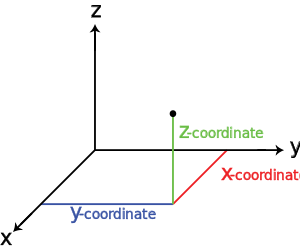
\includegraphics[scale=1]{R3}
	\end{figure}
	 
	 توجه کنید که در بعضی از نرم افزارها جای $  Y $ با $ Z $ عوض میشود.
	 
	یک بردار را در فضای $ R^3 $ به صورت زیر نشان میدهیم:
\[  \vec{V} = \begin{pmatrix}
X \\
Y \\
Z
\end{pmatrix}  \]
	 همه ی قوانین $ R^2 $ برای  $ R^3 $ برقرار است. مثلا به بردار واحد محور $ Z $، $ \vec{k} $ میگویند. غرض از این بخش، اینست که \textbf{قائمیت}\footnote{ Orthogonality} در فضای سه بعدی را معرفی کنم. زیرا برای بازیهای دو و نیم بعدی، دوربین باید قائم بر فضای $ R^3 $ باشد.
	 
	 

	 \begin{figure}[H]
	 	\centering
	 		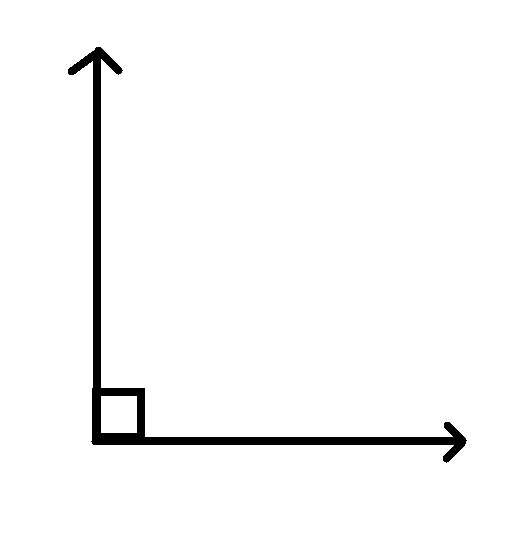
\includegraphics[scale=0.3]{Orthogonal}
	 \end{figure}

	 در کل، دو بردار وقتی بر هم قائمند که حاصلضرب نقطه ای آندو، صفر باشد:
	 \[ \vec{A} \text{قائم است بر } \vec{B} \text{اکر و تنها اگر} \vec{A}.\vec{B} = 0 \]  
	 
	 اگر فرمول ضرب نقطه ای یادتان باشد، و در اینترنت کسینوس 90 را خوانده باشید، میدانید که:
	 
	 
	 
	 \[ \vec{A}.\vec{B} = |A||B|\cos \alpha \]
	 
	 و $ \ cos(90)  = 0$
	 پس:
	 
	 \[ |A||B|\cos (90) = 0 \ \]
	 
	 
\section{پایان فصل ریاضی}\label{mathend}

کلید یادگرفتن ریاضی یک چیز است: $  \text{تمرین}^n  $! یادتان نرود که حافظه، چیزیست فرَار، و هر لحظه ممکن است همین چیزهای کمی که از بنده ی حفیر آموخته اید، که مطمئنم برای بیشتر شما یک یادآوری ساده و کوتاه بوده، و برای خیل عظیمی از شما فوت آب بوده، و فقط یک لیست است، سریع از حافظه ی شما رخت برمیبندند. تمرین کنید، نوت برداری کنید، و یادتان نرود که روم را در یک روز نساخته اند. این ضرب المثال را چندین بار در طول کتاب تکرار خواهم کرد. یادگیری طول میکشد. و یادتان نرود که هیچکس استعداد چیزی را ندارد، و همه چیز با تمرین میسر میشود.

در فصل بعد، در مورد برنامه نویسی، زبان پایتان و \lr{C++} حرف خواهیم زد.
	 
	   
	 \chapter{نگاهی کوتاه به برنامه نویسی}\label{programming}
	 
	 درین فصل نگاهی کوتاه می اندازیم به \textbf{برنامه نویسی}\footnote{Programming}. ابتدا به دو \textbf{پَرَدایم}\footnote{Paradigm} برنامه نویسی \textbf{فانکشنال}\footnote{Functional} و \textbf{شیء گرا}\footnote{\lr{Object Oriented Programming}}. و بعد \textbf{پیچیدگی زمانی}\footnote{\lr{Time Complexity}} را توضیح خواهیم داد. بعد از آن، نگاهی می اندازیم به \textbf{سینتکسِ}\footnote{به دستور زبانی یک زبان برنامه نویسی Syntax گفته میشود.} زبان \textbf{پایتان}\footnote{Python} و \textbf{\lr{C++}}.
	 
\section{برنامه نویسی فانکشنال}\label{functional}

از بین تمام روشها، یا به عبارتی، پَرَدایمهای برنامه نویسی، برنامه نوسی فانکشنال یا \textit{تابعی} ساده ترین، و پر مصرف ترین آنهاست. اکثر اشخاصی که برنامه نویسی را شروع میکنند، از برنامه نویسی فانکشنال شروع میکنند. زبانهای قدیمی مانند \textbf{فورترن}\footnote{FORTRAN}	و \textbf{لیسپ}\footnote{Lisp} همه فانکشنال هستند. 

با توابع در فصل ریاضی آشنا شدیم. توابع کامپیوتری نیز با توابع ریاضی فرق زیادی ندارد، همه ی آنها یک ماشین هستند که ورودی را به خروجی تبدیل میکنند. یک تابع، مجموعه ای از \textbf{دستورات}\footnote{Instructions} است که \textbf{پارامتر}\footnote{Parameter} داده شده را با تغییرات، باز میگردانند. این تغییرات میتواند عملیاتهای جمع و تفری، ضرب و تقسیم، باقیمانده، و یا تغییر نوع پارامتر مثلا از عدد صحیح به عدد حقیقی، و یا هرچیز دیگری باشد. برای اجرای تابع، آنرا \textbf{میخوانیم}\footnote{Call} و به پارامتری که به آن میدهیم، \textbf{آرگومان}\footnote{Argument} میگوییم.

اینستراکشن سِت زیر را در نظر بگیرید:

\begin{enumerate}
	\item عدد $ n $ را بگیر.
	\item برای $ n $ بار، $ n $ را ضربدر $n - 1$ کن.
	\item جواب را برگردان.

\end{enumerate}

به این تابع، تابع \textbf{فاکتوریل}\footnote{Factorial} میگویند. توابع زیادی هستند، پیچیده و ساده، مهم اینجاست که از آنها درست استفاده کنید. 
بعضی از توابع، پارامتر قبول نمیکنند. بعضی از توابع، ارزشی را باز نمی گردانند. به این نوع از توابع \textbf{ووید}\footnote{Void} میگویند. بعضی از زبانها، \textbf{تایپ ثابت}\footnote{\lr{Statically Typed}} هستند و باید نوع ارزشهای باز گرداننده را مشخص کرد. \lr{C++} یکی ازین نوع زبانهاست. بعضی از زبانها \textbf{تایپ دینامیک}\footnote{\lr{Dynamically Typed}} هستند و لازم نیست نوع ارزش بازگرداننده را در آنها مشخص کرد. پایتان یکی ازین زبانهاست. هردو زبان پایتان و \lr{C++} هم فانکشنال هستند، هم شیء گرا. در مورد پَرَدایم شیء گرا در بخش بعد صحبت خواهیم کرد. 
هرزبان مقداری تابع از پیش تغیین شده دارد، اما بقیه ی تابع ها را خودتان باید تعیین کنید. اینکه در چه زمانی باید تابع تعیین کرد، قانون طلایی اینست که هرگاه دیدید عملی را دارید بیشتر از یک بار انجام میدهید، وقت تعیین کردن یک تابع است. 
همه ی زبانها دارای \textbf{کتابخانه}\footnote{Library} هایی هستند که شامل توابع و کلاسها \(\ref{oop}\) و دیگر کدهایی هستند که به برنامه نویس کمک میکنند خود را تکرار نکند.
 
	 
	\textbf{خود را تکرار نکنید.}\footnote{\lr{DRY - Don't Repeat Yourself}}
	
	قانون پلاتینیوم برنامه نویسی، اینست. هرگز چیزی که در یک کتابخانه موجود است را ننویسید. مثلا عوض اینکه در زبان \textbf{جاوا}\footnote{Java} عوض نوشتن صدها خط کد برای به دست آوردن یک تابع ماتریس، میتوان از کتابخانه ی JAMA استفاده کرد.
	
	
	
	
	
	
	 
	 \section{برنامه نویسی شیء گرا}\label{oop}
	 
	 
	 برنامه نویسی شیء گرا بر پایه ی کانسپتِ \textbf{کلاس}\footnote{Classes} میجرخد.
	 
	 گفتیم توابع مانند ماشینهایی هستند که اطلاعات را از حالتی به حالت دیگر تغییر میدهند. اگر تابع، ماشین است، کلاس، یک خیابان پر از ماشین است که در آن هزاران ماشین وجود دارد، و همچنین چندده هزار عابر پیاده که سوار ماشین میشوند. درین تشبیه، به ماشین \textbf{اسلوب}\footnote{Method} و به عابر پیاده \textbf{خواص}\footnote{Properties} میگویند. اگر ایده ی کلاس، یعنی یک خیابان پر از عابر پیاده و ماشین \(به ترتیب، اسلوب و خواص\) را داشته باشیم، با آن میتوانیم هزاران هزار خیابان بسازیم. به هر خیابانی که ما میسازیم، \textbf{شیء}\footnote{Object} میگویند. در یک کتابخانه مانند کتابخانه ی JAMA که از آن نام بردیم، یک کلاس به نام ماتریس وجود دارد و این کلاس چندین اسلوب و چندین خواص دارد. یکی از آن اسلوبها، ارزش سطر و ستون داده شده را به کاربر برمیگرداند.
	 بعضی از متدها و خواصها، خصوصی اند، یعنی جز سازنده ی کلاس خیابان، کسی اجازه ی عوض کردن آن را ندارد. اما بعضی از اسلوبها و متدها قابل تغییرند.
	 فرض کنیم یک کلاس داریم به نام مدرسه. برای ساختن یک شیء مدرسه از آن، باید به آن \textit{ارزشهایی} مانند آدرس مدرسه، تعداد کلاسها، اینکه مدرسه بوفه داشته باشد یا نه، نام مدرسه، اینکه دبیرستان است یا ابتدایی، و... را بدهیم تا از آنها، \textit{خواص} مدرسه را تعیین کند. این کار توسط اسلوب \textbf{سازنده} \footnote{Constructor} انجام میشود. و یا به سادگی میخواهیم یک مدرسه ی قدیمی را بکوبیم و خراب کنیم. برای این کار از اسلوبی به نام \textbf{خراب کننده}\footnote{Destructor} استفاده میکنیم. 
	 یگ گلاس میتواند چنین سازنده داشته باشد، ولی فقط یک خراب کننده میتواند داشته باشد.
	 
	 در بخش بعدی در مورد کتابخانه ها صحبت خواهیم کرد.
	 
	 \section{کتابخانه ها}\label{lib}
	 
	 به مجموعه توابع و کلاسهای از قبل آماده شده، کتابخانه میگویند.
	 هر کدی که در صورت اجرا، عملیات خاصی انجام نداده، و به کدهای دیگر برای اجرا وابسته باشد، کتابخانه نام میگیرد.
	 اکثر زبانها برای کتابخانه های خود دارای یک دیتابیس هستند، که زبان پایتان جزء آنهاست، اما بعضی از زبانها برای کتابخانه های خود دیتابیس ندارد، مانند \lr{C++}. دلیل آن اینست که اکثر کتابخانه های \lr{C++}، متن بسته و پولی هستند.
	 کتابخانه ها میتوانند به صورت فایل متنی، یا فایل \textbf{باینری}\footnote{Binary} عرضه شوند. کتابخانه های پایتان متنی، و کتابخانه های \lr{C++} باینری هستند. گاها کتابخانه هایی به صورت متنی نیز عرضه میشوند.
	 در این کتاب آموزش ساخت یک کتابخانه ی برنامه نویسی خلاقانه با پایتان را خواهیم داد.
	 
	 \section{پایتان}\label{py}
	 
	 زبان پایتان در سال 1999 برای بار اول عرضه شد و در هنگام نوشتن این کتاب، در ورژن 3.7.1 به سر میبرد. درین فصل، فقط قطره ای از دریای این زبان را آموزش میدهیم. برای آموزش بهتر زبان، به کتاب مخصوص مراجعه کنید.
	 
	 پایتان زبانی کاملا مدرن، قابل انعطاف، یکدست، و جذاب و ساده میباشد که برای از اتوماسیون گرفته تا بازی سازی، کاربرد دارد. 
	 اینستراکشن های پایتان \textbf{ترجمه}\footnote{Interpret} میشوند، یعنی لازم نیست که از قبل به زبان اسمبلی یا ماشین در بیایند، بلکه، در حین اجرا به زبانهایی مثل C یا Java ترجمه میشوند و بعد خط به خط اجرا میشوند. عرضه ی اصلی پایتان که ما از آن استفاده میکنیم، از \lr{C++} استفاده میکند.
	 
	\subsection{نصب پایتان}\label{pyinstall}
\begin{enumerate}
	\item به این صفحه بروید و پایتان را دانلود کنید: \url{https://www.python.org/downloads/}
	\item آنرا نصب کنید.
	\item از فایل اکسپلورر مانند زیر روی Properties کلیک کنید:
		 \begin{center}
		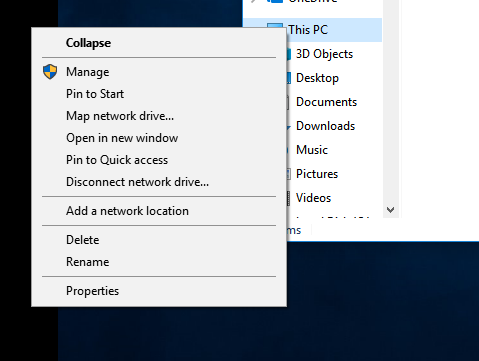
\includegraphics[scale=1]{InstallPython_1}
	\end{center}
	\item  روی \lr{Advanced System Settigns} کلیک کنید.
	\begin{center}
		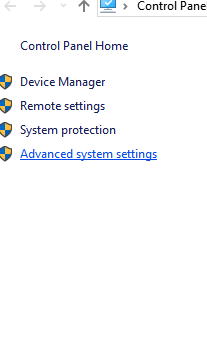
\includegraphics[scale=1]{InstallPython_2}
	\end{center}
\item روی گزینه \lr{Environment Variables} کلیک کنید.
\begin{center}
	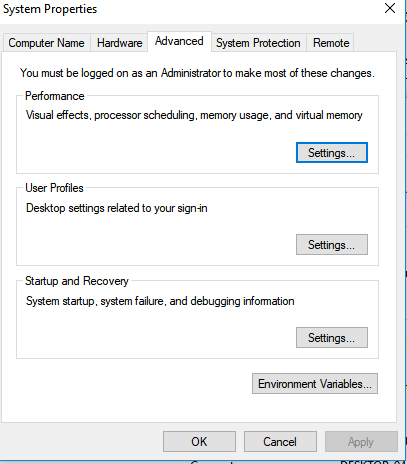
\includegraphics[scale=1]{InstallPython_3}
\end{center}
\item روی Path  کلیک کنید.
\begin{center}
	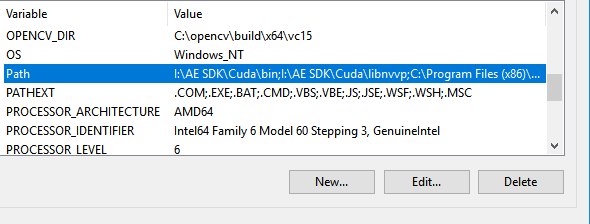
\includegraphics[scale=1]{InstallPython_4}
\end{center}
\item دو گزینه ی زیر را به آن اضافه کنید.
\begin{center}
	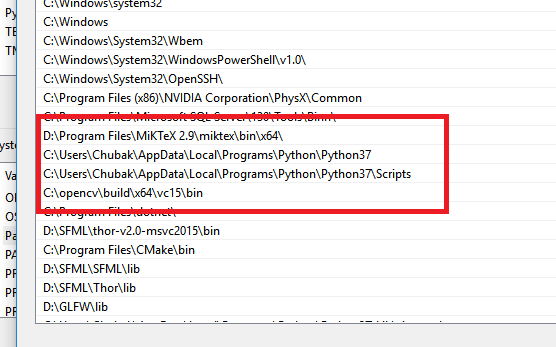
\includegraphics[scale=1]{InstallPython_5}
\end{center}
\end{enumerate}
	 
	 برای نوشتن کد پایتان احتیاج به یک \textbf{محیط گسترش مجتمع]}\footnote{Integrated Development Environment} دارید. من \lr{PyCharm Community} را پیشنهاد میکنم که کاملا مجانیست. آنرا میتوانید از \url{https://www.jetbrains.com/pycharm/download/#section=windows} دانلود کنید. 
	 بعد از باز کردن پای چارم و باز کردن یک پروژه ی جدید، از طریق زیر یک فایل پایتان بسازید:
	 
	 \begin{center}
	 	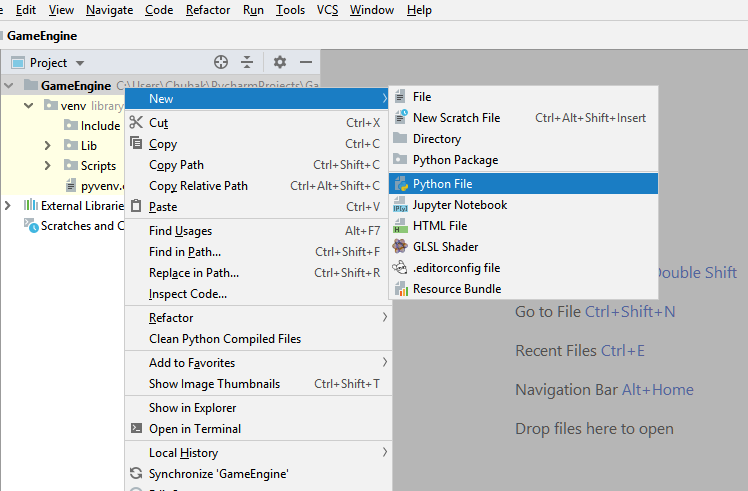
\includegraphics[scale=0.6]{CreateNewPythonFile}
	 	\end{center}
 	
 	حال وقت نوشتن اولین کد ماست. بنویسید:
 	
 	
 	\begin{latin}
 	\mono{	\begin{lstlisting}
new_variable = "A Portal to the World of Python"
print(new_variable)
 		\end{lstlisting}}
 	
 \end{latin}
و \lr{\keys{\ctrl + \shift + F10}}  را بزنید. در پایین صفحه، کد شما اجرا میشود.
\begin{tip}
	میتوانید از محیطهای گسترش دیگر نیز استفاده کنید. مانند \lr{Beans IDE}، PyDev، SpyDer، \lr{Cloud9 IDE}و درضمن، \lr{Microsoft Visual Studio} نیز یک پکیج پایتان دارد.
\end{tip}


	 
	 
	 
	 \subsection{متغیرها}\label{vars}
	 در بخش قبل، \lr{\mono\lstinline|new_variable|} یک \textbf{متغیر}\footnote{Variable} است. ممتغیرها مانند ظروفی هستند که میتوان در آنها هر چیزی ریخت. چون پایتان زبان \textbf{تایپ امن}\footnote{\lr{Type Safe}} \textit{نیست}، میتوان هر نوع دیتایی را داخل یک متغیر جا داد.
	 
	 
	 	\begin{latin}
	 		
	 	\mono{	\begin{lstlisting}
var = True #boolean
var = "String" #string
var = 1 #integer
var = 1.0 #float	
var = Class() #Class
	 		
	 		
	 		\end{lstlisting}} \end{latin}
	 
	 همانطور که میبینید، متغیرهای پایتان هر \textbf{نوع دیتایی }\footnote{دیتا تایپ} را قبول میکنند، استرینگ، عدد صحیح، فلوت و کِلس. بگذارید تمام این انواع دیتا را توضیح دهم.
	 
	 \begin{itemize}
	 	\item به متغیرهایی که دو حالت \textbf{راست}\footnote{True} و \textbf{غلط}\footnote{False} دارند، متغیر \textbf{بولی}\footnote{Boolean} میگویند.
	 	\item به تکه های متنی که از الفباء تشکیل شده، \textbf{رشته} یا String میگویند. به متنی که به یک استرینگ میدهیم، \textbf{لیترال}\footnote{Literal} میگویند.
	 	\item  به اعداد صحیح بدون اعشار \textbf{اینتجر}\footnote{Integer} یا به کوتاه int میگویند.
	 	\item به عدد حقیق با اعشار \textbf{float}\footnote{Float} میگویند
	 	\item از هر کلاصی می توان یک متفیر ساخت. درین صورت، نام کلاس، نوع متغیر میشود.
	 \end{itemize}
 
 اینها فقط چند نوع از متغیرهای پایتان هستند. همانطور که گفته شد، لازم نیست نوع متفیر را مشخص کنید چون پایتان، تایپ امن نیست. اما لازم است برای تعیین نوع آن، آنرا \textbf{مقداردهی اولیه}\footnote{Initialize} نمایید.
	 
	 
	اما اگر بخواهیم چندین نوع دیتا، یا متغیر، را در یک متغیر نگاه داریم چه؟ بخش \ref{list} درین مورد صحبت خواهد کرد.
	
	\subsection{لیست، تاپل، دیکشنری}\label{list}
	 
	 برای نگاه داشتن چندین نوع دیتا، یا چندین متغیر، در یک مکان، از \textbf{لیست}\footnote{Lists} استفاده میکنیم.لیستها به صورت زیر مقداردهی اولیه میشوند:
	 
	  	\begin{latin}
	 	\mono{	\begin{lstlisting}
a_list = []
a_list = [1, 2, 3, 4]
a_list = ["Hello World", "Goodbye World"]
a_list = [1, 2, 3, 4, "Hello", "World"]
	 		\end{lstlisting}}
	 	
	 	\end{latin}
	 		
	 		یک لیست وقتی مقداردهی اولیه شد، نباید با علامت مساوی، به آن مقدار اضافه کرد. بلکه، باید از \lr{\mono\lstinline|list.append|} استفاده کرد:
	 	\begin{latin}
	 	\mono{	\begin{lstlisting}
a_list = [1]
print(a_list)
a_list.append(2)
print(a_list)
	 		\end{lstlisting}}
	 			
	 	\end{latin}
 		
 \lr{\keys{\ctrl + \shift + F10}} را بزنید تا نتیجه را ببینید.
 		در زیر چند اسلوب لیست را میخوانید.
 		\begin{itemize}
 			\item \lr{\mono\lstinline|list.reverse|}: لیست را برعکس یا به بعیارت دیگر، معکوس میکند.
 			\item  \lr{\mono\lstinline|list.copy|} لیست را در لیست دیگر کپی میکند.
 			\item  \lr{\mono\lstinline|list.pop|} در \textbf{ایندکس}\footnote{Index - به شماره ی عضو ایندکس میگویند.} داده شده، عضو را پاک میکند.
 			\item \lr{\mono\lstinline|list.sort|} لیست را بر اساس الگوریتم \textbf{\lr{Merge Sort}} مرتب میکند.
 			\item  \lr{\mono\lstinline|len(list)|} سایز لیست را به دست می اورد.
 		\end{itemize}
 		
	 		
	 یک لیست، میتواند لیستهای دیگری نیز در بر بگیرد:
	 
	 
	 	\begin{latin}
	 	\mono{	\begin{lstlisting}
multi_dimensional_list = [[], [], []]
multi_dimensional_list.append([])
	 		\end{lstlisting}}
	 	
	 \end{latin}
 
 برای به دست آوردن عضو خاصی از لیست، از ایندکس آن استفاده میکنیم.
 
 	 	\begin{latin}
 	\mono{	\begin{lstlisting}
 my_list = [2, 4, 6, 8, 10]
 print(my_list[0])
 		\end{lstlisting}}
 	
 \end{latin}
\textbf{ایندکسها از 0 شروع میشوند} تا سایز لیست منهای یک ادامه دارند. برای بدست آوردن چندین عضو از لیست، از علامت دو نقطه استفاده میکنیم:

 	 	\begin{latin}
	\mono{	\begin{lstlisting}
my_list = [2, 4, 6, 8, 10]
print(my_list[0:3])
		\end{lstlisting}}
	
\end{latin}

 	 
	 در کل، لیستها بهترین روش برای نگه داشتن دیتاهای زیاد هستند. اما برای دیتای کم و \textbf{غیر جهشی}\footnote{Immutable}، از \textbf{تاپل}\footnote{Tuple} استفاده میکنیم.  تاپلها میتوانند به اندازه ی لیست دیتا نگه دارند، اما نمیتوان از آنها دیتا کم و زیاد کرد. تاپلها بدین صورت تعریف مقداردهی اولیه میشوند:
	 
	 
 	 	\begin{latin}
	\mono{	\begin{lstlisting}
my_tuple = (R, G, B)
print(my_tupe[0:1])
		\end{lstlisting}}
	
\end{latin}
	 مقلا برای رنگ یا موقیت یک فرگمنت در یک تصویر رَستر \(در مورد اینها مفصل صحبت خواهیم کرد\) از تاپل استفاده میشود. مانند لیستها، میتوان از \lr{\mono\lstinline|len()|} برای بدست آوردن سایز تاپل استفاده کرد.
	 
	 دیکشنریها نیز مانند لیستها، برای نگه داشتن مقدار زیادی دیتا استفاده میشود. اما در دیکشنری، ایندکسها، عوض شماره، دارای نام هستند \(میتوان از شماره نیز استفاده کرد\). دیکشنریها \textbf{همتا به همتا}\footnote{Peer to Peer} هستند. برای مقداردهی اولیه ی یک دیکشنری، از سینتکس زیر استفاده میکنیم:
	 
	 \begin{latin}
	 	\mono{	\begin{lstlisting}
my_dict = {"Name" : "Chubak",
	"Last Name" : "Bidpaa"}
print(my_dict["Name"])
	 	\end{lstlisting}}
	 	
	 \end{latin}
	 
	 \begin{tip}
	 	در تمام زبانهای برنامه نویسی، زدن \keys{\return}  وسط خط کد اشکالی ندارد.
	 \end{tip}
	 
	 
	 مهمترین اسلوب دیکشنری \lr{\mono\lstinline|dictionary.items()|} میباشد که آیتم های دیکشنری را برمیگرداند. در بخش لوپ در موردش صحبت خواهیم کرد صحبت از لوپ شد، وقت آن است که در مورد \textbf{بیانیه های}\footnote{Statements} پایتان صحبت کنیم.
	 
	 \subsection{بیانیه های شرطی}\label{pyif}
	 
	 
	 \textbf{بیانیه های شرطی}\footnote{\lr{Conditional Statements}}، بخشهایی از پایتان هستند که به کد اجازه ی اجرا، یا در صورت عدم اجازه، اجازه ی اجرای کد دیگری را میدهند.
	 
	 \textbf{کلمات کلیدی}\footnote{Keywords} که ما برای شرط گذاشتن روی جریان اجرای برنامه استفاده میکنیم، \textbf{if} و \textbf{else} و \textbf{elif} هستند. همیشه لازم نیست از دوتای دوم استفاده کرد، اما پیشنهاد میشود اگر مستلزم است، حتما از آنها استفاده کنید. کد زیر را ببینید:
	 
	 
	 \begin{latin}
	\mono{	\begin{lstlisting}
pi = 3.14
r = 10
area= pi*r*r
		
if area > 20:
	print("The area is greater than 20.")
else:
	print("The area is not greater than 20.")
		
		\end{lstlisting}}
	
\end{latin} 
	 
	این کد، مساحت یک دایره با شعاع 10 را حساب میکند و  اگر این مساحت، بیشتر از 20 است، میگوید مساحت بیشتر از 20 است، وگرنه میگوید مساحت بیشتر از 20 نیست. به همین سادگی، ما \textbf{جریان}\footnote{\lr{Execution Flow}} اجرای کد را تغییر دادیم. 
	
	\begin{tip}
		پای چارم خودش اینکار را میکند، اما بین اول خط کلمه ی if و else و \textbf{اصطلاح}\footnote{Expression} شرط، باید چهار \keys{\space} فاصله باشد.
	\end{tip}


برای شرط کذاشتن، از \textbf{آپریتور}\footnote{Operator} هایی مانند $ < $ استفاده میکنیم. به اعدادی که آپریتور روی آنها تاثیر میگذارد، \textbf{آپرَند}\footnote{Operand} میگویند.

آپریتور های شرطی پایتان به شرح زیرند:
	 
	 
	
	\begin{table}[H]\label{pyop}
		\centering
		\begin{tabular}{|l|l|}
			\hline
			+               & بعلاوه       \\ \hline
			-               & منها         \\ \hline
			*               & ضرب          \\ \hline
			/               & تقسیم        \\ \hline
			\%              & باقیمانده    \\ \hline
			\textgreater{}  & بزرگتر       \\ \hline
			\textless{}     & کوچکتر       \\ \hline
			\textgreater{}= & بزرگتر مساوی \\ \hline
			\textless{}=    & کوچکتر مساوی \\ \hline
			==              & مساوی        \\ \hline
			!=              & نا مساوی     \\ \hline
			and             & وَ           \\ \hline
			or              & یا           \\ \hline
		\end{tabular}
		\caption{آپریتورهای پایتان}
	\end{table}
			


	 
	 
	 آپریتورهای دیگری نیز داریم مانند آپریتورهای \textbf{Bit-wise} ولی الان به کار ما نمی آیند.
	 
	 میتوانید از کلمه ی کلیدی elif که مخفف Else If است برای افزایش شروط استفاده کنید:
	 
	 
	 \begin{latin}
	\mono{	\begin{lstlisting}
if area > 20:
	 print("The area is bigger than 20.")
elif (area < 15):
	 print("The area is less than 15")
elif area < 10:
	 print("The area is less than 10")
else:
	 print("The area is not bigger than 20.")
	
		
		\end{lstlisting}}	 
	 
\end{latin}

اما این فقط تنها بیانه ی شرطی پایتان نیست. دو بیانیه ی شرطی دیگر داریم، که با if فرق زیادی دارند.



\begin{tip}
	شرط، میتواند یک متغیر بولی باشد. مثلا \lr{\mono\lstinline| bool = 1 < 10|}. این متغیر، راست $\text{(True)}\ $ میباشد چون 1 کوچکتر از 10 است.
\end{tip}


\subsection{بیانیه های چرخشی شرطی}\label{pyloops}
	 
	 بیانیه های \textbf{چرخشی شرطی}\footnote{\lr{Conditional Loops}} بیانیه هایی هستند که تا شرط برقرار است، یک اصطلاح یا بیانیه را به صورت \textbf{نا محدود}\footnote{Indefinitely} اجرا میکنند. گاهی این چرخش، بینهایت است. اما اکثر اوقات، شرط تمام شده و \textit{غلط} $\text{(False))}  $میشود. وقتی شرط، غلط میشود، چرخش تمام شده و بیانیه ی بعدی اجرا میشود. همچنین میتوانیم خودمان جریان چرخش را کنترل کرده، و به میل خود چرخش را تکرار کرده و یا بشکنیم.
	 
	 دو کلمه ی کلیدی برای اینکار استفاده میشود، for و while. اولی مصارف دیگری هم دارد که به آن میپردازیم. اما بگذارید اول به while بپردازیم. سینتکس آن اینگونه است:
	 
	 
	 
	 
	 \begin{latin}
	\mono{	\begin{lstlisting}
		i = 0
		
while i < 50:
	print(str(i))
	i += 1
		
		\end{lstlisting}}	 
	
\end{latin}
	 
	 
	ابتدا ما به متغیر  \lr{\mono\lstinline|i|} عدد 0 را میدهیم. بعد میگوییم تا این متغیر، از 50 کوچکتر از، ارزش متغیر را روی صفحه نمایش بده و در هر \textbf{بازتکرار}\footnote{Iteration}، ارزش 1 را به متغیر اضافه میکنیم. وقتی متغیر به 50 رسید، چرخش تمام میشود و به بیانیه ی بعدی میرسد. 
	
	\begin{tip}
	تابع \lr{\mono\lstinline|print()|} نمیتواند جز استرینگ لیترال و استرینگ، چیز دیگری را در صفحه به نمایش بگذارد. با استفاده از تابع  \lr{ \mono\lstinline|str()| } متغیرهای عددی را به استرینگ لیترال تبدیل میکنیم.
	\end{tip}
	 
	 
	 
	 
	 میتوانید با استفاده از کلمه ی کلیدی \lr{\mono\lstinline|and| } یک شرط دیگر اضافه کنید:
	 
	 \begin{latin}
	\mono{	\begin{lstlisting}
i = 0
		
while i < 50 and i < 25:
	print(str(i))
	i += 1
		
		\end{lstlisting}}	 
	
\end{latin}
	 
	 
	 اینگونه، فقط در صورتی متغیر روی صفحه پرینت میشود که بین 25 و 50 باشد. \lr{\mono\lstinline|or|} هم دو یا چند شرط را در صورتی اجرا میکند که یکی از آنها، راست باشد. 
	 
	 کلمه ی کلیدی بعدی که داریم، for میباشد. این کلمه بیشتر برای دسترسی به لیست، دیکشنری و تاپل به کار میرود \(\ref{iterter}\) اما برای چرخش برای n بار از سینتکس زیر استفاده میکنیم:
	 
	 
	 
	 
	 	 
\begin{latin}
	 	\mono{	\begin{lstlisting}
for i in range(n):
	print(str(i))
	 		
	 		\end{lstlisting}}	 
	 	
	 \end{latin}
	 
	 
	 
	 تابع  \lr{\mono\lstinline|range(m, n)|} یک لیست قابل بازتکرار بین m و n ایجاد میکند. اگر پارامتر اول را به آن ندهیم، یک لیست قابل بازتکرار بین 0 و n ایجاد میکند. و متغیر ارزش i را در هر بازتکرار، بر اساس لیست ساخته شده مشخص میکند. این بیانیه ی چرخشی شرطی نیست، بلکه بیانیه ی چرخشی بازتکراریست. در بخش بعد، از کلمه ی کلیدی for برای دسترسی به اعضای لیست، تاپل، و دیکشنری استفاده میکنیم.
	 
	 
\subsection{دسترسی به لیست، دیکشنری و تاپل}\label{iter}
	 
	 برای دسترسی به اعضای یک لیست، تاپل، دیکشنری، یا هر شیء \textbf{قابل بازتکرار}\footnote{Iterable} دیگری، از for استفاده میکنیم. مثال برای لیست اینگونه است:
	 
	 \begin{latin}
	 	\mono{	\begin{lstlisting}
one_dim_list = [1, 2, 3]
two_dim_list = [[1, 2, 3], [4, 5, 6]]
	 		
for i in one_dim_list:
	  print(i)
	 		
	 		
for list in two_dim_list:
	 for i in list:
	 print(i)
	 		\end{lstlisting}}	 
	 	
	 \end{latin}
	 
	 
	 
	 
	 همانطور که مشاهده میکنید، ما با استفاده از کلمه ی کلیدی in توانستیم به اعضای لیست یک بعدی \lr{\mono\lstinline|one_dim_list|} دسترسی پیدا کنیم و آنها را روی صفحه پرینت کنیم. سپس، ما با استفاده از یک بیانیه ی \textbf{لانه ای}\footnote{\lr{Nested Statement}} توانستیم یک لیست دو بعدی را روی صفحه پرینت بگیریم.
	 
	 \begin{tip}
	 	تمام بیانیه های چرخشی را میتوان لانه کرد، اما اگر که اشتباهی صورت بگیرد، \textbf{سرریزی پشته}\footnote{\lr{Stack Overflo}} صورت میپذیرد. پشته بخشی از زبان C است که کامپایلر پایتان در آن نوشته شده است.  \ref*{refpointer} را بخوانید.
	 \end{tip}
	 
	 
	 ما میتوانیم با استفاده از دو کلمه ی کلیدی break و continue بر جریان چرخشمان تاثیر بگذاریم.
	 
	 

		 	 \begin{latin}
			\mono{	\begin{lstlisting}
n = 0
while True:
	n += 1
				
	if (n > 20):
		break;
				\end{lstlisting}}	 
			
		\end{latin}

	 
	 
	 این کد، همیشه صحیح است، پس همواره اجرا میشود. اما اگر متغیر ما، بیشتر از 20 شود، زنجیر میشکند و چرخش پایان میابد. continue نیز مانند break است، فقط حلقه را نمیشکند، بلکه کاری میکند که حلقه دوباره بازتکرار شود.
	 
	 
	 
	\subsection{تابع در پایتان}\label{pyfunc}
	در بخش پَرَدایم فانکشنال، در مورد توابع در برنامه نویسی صحبت کردیم. در پایتان، تابع بلوکه ای از کد است که با خواندن آن، یک یا یک امر صورت میپذیرد، یا یک ارزش باز گردانده میشود، یا هردو. پایتان دارای 68 تابع از پیش ساخته شده است، و ما خودمان میتوانیم تا هرچقدر لازم داریم، تابع بسازیم. برای اینکار، از کلمه ی کلیدی def استفاده میکنیم:
	 
	 
	 \begin{latin}
	\mono{	\begin{lstlisting}
def first_functions():
	pi = 3.14
	r = 10
	area = pi * r * r
		
	print(area)
		
		
	def second_function(r):
	   pi = 3.14		    
	   area = pi * r * r
		
		    return area
		\end{lstlisting}}	 
	
\end{latin}


	 
همانطور که مشاهده میکنید، تابع اولی، نه پارامتر قبول میکند، نه ارزشی را باز میکرداند. اما یک عملیات پرینت انجام میدهد. به این نوع توابع، همانطور که گفتیم، ووید میگویند.

تابع دوم یک تابع فلوت است، چون یک ارزش فلوت باز میکرداند. و ابتدا شعاع دایره را به عنوان پارامتر میپذیرد.

یک تابع را میتوان در خودش بخواند. به این امر \textbf{تابع بازگشتی}\footnote{\lr{Recursive Function}} میگویند. مثلا برای بدست آوردن فاکتوریل یک عدد:



	 
	 
	 \begin{latin}
	\mono{	\begin{lstlisting}
def factorial(n):
	if n == 1:
		return n
		else:
		return n*factorial(n - 1)
		\end{lstlisting}}	 
	
\end{latin}
	 
	 
	 اگر شرایط بازگشت در تابع محیا نباشد همانطور که در بخش قبل گفتیم، سرریزی پشته صورت میگیرد. در مورد پشته و هرم در بخش \lr{C++} صحبت خواهیم کرد. تا این حد بدانید که پایتان، \textbf{مدیریت حافظه}\footnote{\lr{Memory Management}} را خودش انجام میدهد و نیازی به این کار توسط شما نیست. در \lr{C++} ما متغیرهایی داریم که به آدرس یک متغیر دیگر در RAM اشاره دارند، اما در پایتان، ما همچین چیزی نداریم.
	 
	 \begin{tip}
	 	توجه داشته باشید که \textbf{اسکوپ}\footnote{Scope} متغیرها در تابع، مخصوص خودشان است. اگر متغیری را در یک تابع تعیین کردید، نمیتوانید آنرا بیرون از تابع استفاده کنید. و همچنین اگر متغیری را داخل یک بلاک بیانیه ی شرطی یا چرخش شرطی تعیین کردید، آن متغیر، بیرون از آن بلاک، ارزشی ندارد.
	 \end{tip}	 
	 
	 
	 \subsection{فایل در پایتان}\label{pyfile}
	 برای باز کردن یک فایل در پایتان، از روش زیر استفاده میکنیم:
	 
	 
	 
	 	 \begin{latin}
	 	\mono{	\begin{lstlisting}
f = open(filename,mode)
	 		\end{lstlisting}}	 
	 	
	 \end{latin}
 
 فایل حتما باید در فولدر اسکریپتی که داریم مینویسم باشد. نام فایل یک استرینگ لیترال است پس باید داخل علامت نقل قول باشد. حالت باز کردن فایل بستگی به عملیاتی که میخواهیم روی فایل انجام دهیم دارد. در جدول زیر، حالات باز کردن فایلها را میبینید:
 
\begin{table}[H]
	\begin{tabular}{|l|l|}
		\hline
		'r' & باز کردن یک فایل متنی برای خواندن                       \\ \hline
		'w' & باز کردن فایل متنی برای نوشتن                           \\ \hline
		'x' & حالت ساخت فایل. اگر فایل وجود دارد، عملیات شکست میخورد. \\ \hline
		'a' & باز کردن فایل برای اضافه کردن متن به فایل.              \\ \hline
		't' & باز کردن در حالت متنی.                                  \\ \hline
		'b' & باز کردن در حالت باینری. برای هر فایلی جز فایل متنی.    \\ \hline
	\end{tabular}
\caption{حالتهای باز کردن فایل در پایتان}
\end{table}
	 
	 میتوانید با علامت بعلاوه، حالتها را با هم ترکیب کنید مثلا \lr{\mono\lstinline|open("scene.jpg", 'w+b')|}.
	 
	 برای بستن فایل از اسلوب \lr{\mono\lstinline|file.close()|} استفاده کنید. نوشتن روی فایلها به صورت زیر انجام میپذیرد:
	 
	 	 	 \begin{latin}
	 	\mono{	\begin{lstlisting}
with open("test.txt",'w',encoding = 'utf-8') as f:
	f.write("my first file\n")
	f.write("This file\n\n")
	 f.write("contains three lines\n")
	 		\end{lstlisting}}	 
	 	
	 \end{latin}
	 
	 \subsection{کلاسهای پایتان}\label{pythonclass}
	 
	 در مورد کلاسها در بخش پردایم شیء گرا حرف زدیم. در پایتان، کلاس مجموعه ای از توابع و متغیرهاست که به آنها اسلوب و خواص میگوییم. یک کلاس میتواند فرزند یک کلاس دیگر باشد. آنگاه کلاس فرزند تمام متدها و خواصهای کلاس مادر را به ارث میبرد. یک کلاس به صورت زیر درست میشود:
	 

	 

	 	 	 	 \begin{latin}
	 	\mono{	\begin{lstlisting}
class Rectangle:
 	def __int__(self, color, filled, width, length):
		self.__color = color
		self.__filled = filled
		self.__width = width
		self.__length = length
	 		
	def get_color(self):
		return self.__color
	 		
	def set_color(self, color):
		return self.__color = color
	 		 
	def is_filled(self):
		self.__filled
	 		
	def set_filled(self, filled):
		return self.__filled
	 		
	def get_area():
		return self.__width * self.__length
	 		\end{lstlisting}}	 
	 	
	 \end{latin}
	 
	 
	 کلاس \lr{\mono\lstinline|rectangle|} دارای یک اسلوب سازنده به نام \lr{\mono\lstinline|__int__|} است که که چهار خواص مستطیل را تعیین میکند. و دارای پنج اسلوب دیگر است که هر کدام یک عمل متفاوت انجام میدهند. برای درست کردن یک فرزند از کلاس مستطیل، کافیست به صورت \lr{\mono\lstinline|class Square(Rectangle)|} عمل کنیم. یکی از کارهایی که میشود در برنامه نویسی شی گرا کرد، \textbf{چند ریخت}\footnote{Polymorphism} کردن است. که عبارتست از تعیین یک متد در کلاس فرزند که نام یک متد در کلاس مادر را دارد، ولی خواصش متفاوت است.
	 
	 
	 
	 \subsection{ماژولها و پکیجهای پایتان}\label{pip}
	 
	 پایتان، به خاطر پکیجهایی $ \text{(یا همان کتابخانه ها)} $ که برایش عرضه میشود، نامدار است.
	 پایتان بدون پکیج، یک زبان متوسط است، مانند Perl، Lua، Ada، Ruby و... اما در به خاطر پکیجهایی که برای این زبان در طول سالها عرضه شده، و سادگی نصب این پکیجها، همه برای کارهای کوجک و بزرگ  به پایتان روی می اورند.
	 
	 فلسفه ی نرم افزار مدیریت پکیج پایتان، یعنی pip --- «خود را تکرار نکنید»\footnote{DRY} است. برای نصب یک پکیج روی پایتان، کافیست:
	 
	 \begin{enumerate}
	 	\item CMD را باز کنید.
	 	\item بنویسید \lr{\mono\lstinline|pip install package-name|}.
	 	\item \keys{\return} را بزنید.
	 	\item پکیج روی سیستم شما نصب خواهد شد.
	 	\begin{center}
	 		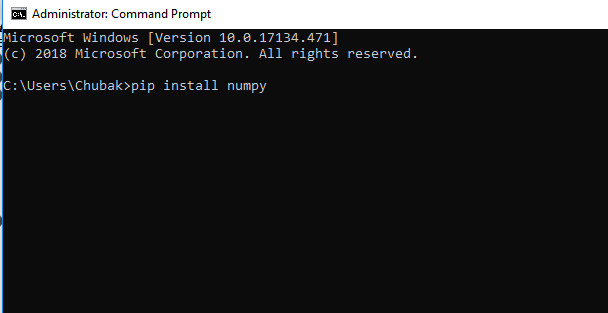
\includegraphics[scale=0.8]{pip_1}
	 	\end{center}
	 \end{enumerate}  
	 
	 
	 وقتی پکیج روی کامپیوترمان نصب شد، میتوانیم با فرمانهای زیر، در اول یا هرجای فایل اسکریپت، پکیج را \textbf{وارد}\footnote{Import} اسکریپتمان کنیم.
	 
	 
	 
	 	 	 \begin{latin}
	 	\mono{	\begin{lstlisting}
import numpy
from numpy import class
import numpy as math
	 		\end{lstlisting}}	 
	 	
	 \end{latin}
 
 چندین نوع وارد کردن وجود دارد. اولی، همانطور که میبینید، وارد کردن کل پکیج است. وقتی اینکار انجام شد. میتوانیم با استفاده از فرمان \lr{\mono\lstinline|numpy.method()|} اسلوبها و خواصهای مورد نظر خود را استفاده نماییم. روش دوم، وارد کردن کلاسی خاص با استفاده از فرمان \lr{\mono\lstinline|from x import y|} است. و فرمان سوم، نام پکیج مورد نظر را تغییر میدهد. 
	 
	 
	 هر پکیج راهنمای خود را دارد که در اینترنت پیدا میشود. در این کتاب، وقتی از یک پکیج نام میبریم، دیگر نمیگوییم آنرا چگونه نصب کنید. وظیفه ی خودتان است که پکیج را نصب کرده و وارد نرم افزار کنید.
	 
	 \subsection{پایان بخش پایتان}
	 
	 با پایان رسیدن بخش پایتان، لازم است یادآوری کنم که من فقط پوسته ی پایتان را خراش دادم. اگر میخواهید بیشتر بدانید، کتابهای متعددی برای اینکار وجود دارند.
	 
	 
	 
	 \section{\lr{C++}}\label{cpp}
	 زبان \lr{C++} در اوایل دهه ی هشتاد توسط دکتر بژورن اشتراشتراپ، مهندس دانمارکی، ابداع شد. فرق \lr{C++} با C در برنامه نویسی شیء گراست. این زبان، عوض پایتان، \textbf{کامپایل}\footnote{Compile} میشود. یعنی، توسط یک نرم افزار به نام کامپایلر که به زبان C نوشته شده، به زبان اسمبلی تبدیل میشود و سپس سیستم عامل انرا به زبان ماشین تبدیل کرده و آنرا اجرا میکند. 
	 
	 
	 کامپایرهای زیادی برای \lr{C++} وجود دارند. دو تا از بزرگترین کامپایلرها، GCC روی لینکس و \lr{Microsoft Visual C++} روی ویندوز است. البته روی ویندوز میتوان از MinGW یا Cygwin هم استفاده کرد.
	  
	 محیط گسترش مچتمع روی ویندوز، برای \lr{C++} زیاد است. اما ما از \lr{Microsoft Visual Studio} استفاده میکنیم. پیشنهاد نمیکنم این نرم افزار را به صورت پایریت شده از بازار بخرید، بلکه، پیشنهاد میکنم نسخه ی مجانی Community آنرا از سایت مایکروسافت دانلود کرده و آنرا نصب کنید.
	 
	 \url{https://visualstudio.microsoft.com/vs/community/}
	  یادتان باشد هنگام نصب، \lr{Visual C++ Tools} را نصب کنید. وگرنه از منوی Tools میتوانید پکیج را نصب کنید. یکی از نیکوییهای ویژوال استودیو، \lr{NuGet Package Manager} است که به شما اجازه میدهد فایلهای \lr{سَری}\footnote{Headers} کتابخانه ها را دانلود کنید. اما ما خودمان فایلهای سَری را دانلود کرده و \textbf{اضافه}\footnote{Include} میکنیم. به معرفی \lr{C++} بپردازیم. چون خیلی از چیزها تکرار از بخش پایتان میباشد، این بخش بسیار کوتاه خواهد بود.
	  
	 برای شروع یک پروژه ی جدید از بخش \lr{File - > New Project} یک پروژه ی \lr{Windows Console Application} بسازید. 
	 
	 \begin{center}
	 	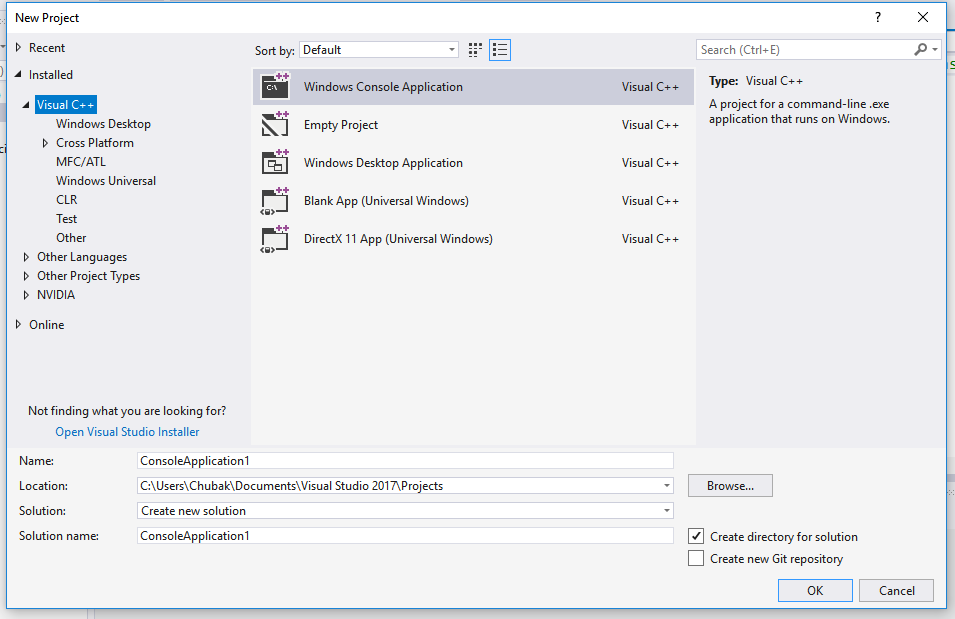
\includegraphics[scale=0.7]{VSNewProject}
	 \end{center}
	 
	 \subsection{سینتکس}\label{cppsyn}
	 
	 یک برنامه ی \lr{C++} به صورت زیر نوشته میشود:
	 
	 	 	 	 \begin{latin}
	 	\mono{	\begin{lstlisting}
#include "pch.h"
#include <iostream>
	 	
int main()
{
	std::cout << "Hello World!\n"; 
}
	 		\end{lstlisting}}	 
	 	
	 \end{latin}
	 
	 کلمه ی کلیدی \lr{\mono\lstinline|#include|} فایلهای سَری برنامه را تعیین میکنند. فایلهای سری، \textbf{اعلامیات}\footnote{Declaration} توابع، متغیرها، و کلاسهای برنامه هستند. \textbf{تعیینات}\footnote{Definitions} برنامه در فایلهای سورس برنامه قرار دارند. هر فایل سری با پسوند .h، یک فایل سورس با همان نام با پسوند .cpp دارد که حاوی تعیینات برنامه است. 
	 
	 تابع \lr{\mono\lstinline|main|} تابع اصلی برنامه است. اگر یک برنامه، تابع اصلی نداشته باشد، کتابخانه به حساب می آید. در \lr{C++} برخلاف پایتان نمیتوانیم یک کد را خارج از تابع به اجرا درآوریم، و تابع اصلی برای همین کار است. 
	 
	 متد \lr{\mono\lstinline|std:cout|} $ \text{(تلفظش سی-اوت میباشد)} $ یکی از اسلوبهای کتابخانه ی \textbf{STL}\footnote{\lr{Standard Template Library}} میباشد. std که با دو تا دونقطه از اسلوب سی-اوت جدا شده، \textbf{فضانام}\footnote{Namespace} اسلوب میباشد.  فضانامها مجمعه ای از اسلوبها هستند که مسمای آنان، کتابخانه شان است. std مسمای اسلوبهای کتابخانه ی STL است.
	 
	 از علامت \lr{\mono\lstinline|>>|} تعجب نکنید، این یک آپریتور بیت وایز میباشد. اما درینجا معنی "خروج" میدهد. با زدن \lr{\keys{\ctrl + F5}} خروجی نرم افزار را خواهید دید.
	 
	 \begin{center}
	 	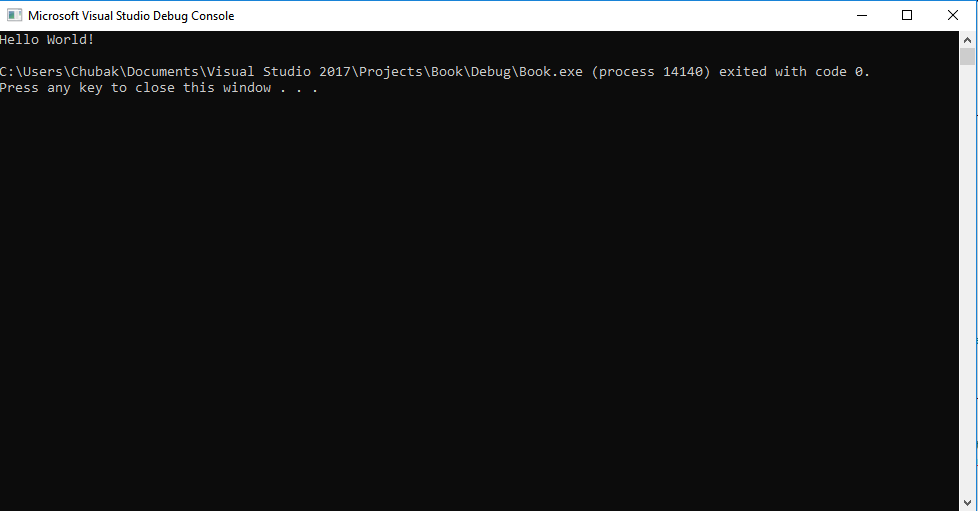
\includegraphics[scale=0.7]{HelloWorld}
	 \end{center}
	 
	 
	 تابع معکوسِ سی-اوت، \lr{\mono\lstinline|std::cin|} $ \text{(سی-این)} $ میباشد. سی-این یک متغیر را گرفته، و به از کیبورد ارزش گرفته و به آن مقداردهی میکند.
	 
	 	 	 	 	 \begin{latin}
	 	\mono{	\begin{lstlisting}
int main()
{
	int variable = 0;
	std::cin >> variable;
	std::cout << variable << std::endl;
}
	 		\end{lstlisting}}
 	
	 	
	 \end{latin}
	 
	 
	 کدِ بالا، توسط سی-این، یک عدد به متغیر میدهد و بعد آنرا به نمایش میگذارد. \lr{\mono\lstinline|std::endl|} که حرف آخرش L کوچک است، خط جدید ایجاد میکند.
	 همانطور که توجه کرده اید، متغیرها در \lr{C++}، نوع دارند چون \lr{C++} زبان تایپ امن است. زیر زیر چند گونه از انواع دیتا در این زبان را مشاهده میکنید.
	 	 	 	 \begin{latin}
	\mono{	\begin{lstlisting}
//integer
unsigned int;
signed int;

unsigned short;
signed short;

unsigned long long;
signed long long;

unsigned long;
signed long;

//decimal
float;
double;
long double;

//text
char;
wchar_t;

//rest
bool;
void;

		\end{lstlisting}}	 
	
\end{latin}
	 
	 
	 
	 تمام اعداد صحیح دو حالت دارند، signed و unsigned. همانطور که بر می آید، اگر یک عدد صحیح signed باشد، میتواند اعداد منقی نیست دریافت کند. اما اگر عدد صحیح unsigned باشد، بین 0 و مکسیمم اعداد صحیح پذیرفته شده توسط پراسسور کامپیوتر است. مکسیمم short، یک عدد بسیار کوچکتر از مکسیمم int بوده، و مکسیمم long و long long بسیار از مکسیمم int بیشترند. اما long و long long، با استفاده از \textbf{حقه های اتاق نشیمن}\footnote{Parlor Tricks} مکسیمم بیشتری دارند. مکسیمم واقعی اعدادی که یک کامپیوتر دریافت میکند، توسط \textbf{واحد پراسسور مرکزی}\footnote{\lr{Central Processing Unit or CPU}} تعیین میشود. مثلا یک پراسسور 32 بیتی میتواند بین -2,147,483,647 و 2,147,483,647 عدد صحیح نگه دارد که مساوی $ 2^31 $ میباشد. یک پراسسور 64 بیتی $ 2^63 $ مکسیمم عدد نگه میدارد. اما معنی 32 بیت و 64 بیت چیست؟ در بخش \ref{refpointer} خواهید خواند. در \lr{C++}، متفیر int، 32 بیتی است. اما در کتابخانه ی استاندارد، int 32 بیتی نیز یافت میشود.
	 
	 متغیرهایی که عدد اعشار میپذیرند،  سه نوعند. فلوت، که در پایتان با آن آشنا شدیم، \textbf{دابل}\footnote{Double} که \textbf{دقت}\footnote{Percision} آن دو برابر فلوت است، و دابل طولانی، که دقتش چندین برابر دابل معمولی است.
	 
	 \begin{tip}
	 	شاید برایتان سوال باشد که از فلوت استفاده کنید یا از دابل. جواب، در احتیاجات شماست. مثلا اگر $ \pi $ را حساب کنیم، و آنرا یک بار در فلوت قرار بدهیم، یکی بار در دابل، یک بار در لانگ دابل:	 		 	 	 	 \begin{latin}
	 		\mono{	\begin{lstlisting}
//float:
3.1415927410125732421875 
//double:
3.141592653589793115997963468544185161590576171875 
//long double:
3.14159265358979323851280895940618620443274267017841339111328125 
	 			\end{lstlisting}}	 
	 		
	 	\end{latin}
	 \end{tip}
	 
	 
	 
	 \lr{\mono\lstinline|char|} و \lr{\mono\lstinline|wchar_t|} انواع کاراکتر در \lr{C++} هستند. اولی، فقط کاراکترهای \textbf{اسکی}\footnote{ASCII - کیبورد استاندارد آمریکا} دومی کاراکتر های \textbf{یونیکد}\footnote{Unicode - کااکتر ستی که تمام کاراکترهای دنیا، حتی خط میخی پارسی، را در بر دارد.} را قبول میکند. میتوان خود کاراکتر را به این متغیر داد، یا شماره ی آن در یونیکد یا اسکی را.
	 
	 در \lr{C++} مانند پایتان، نوع استرینگ نداریم. اما در کتابخانه ی استاندارد استرینگ داریم که \lr{\mono\lstinline|std::string|} نام دارد. برای استفاده از بخش استرینگِ کتابخانه ی استاندارد مانند زیر عمل میکنیم:
	 
	 
	 
	 	 		 	 	 	 \begin{latin}
	 	\mono{	\begin{lstlisting}
#include <iostream>
#include <string>

int main()
{
	std::string myString = "Text";
}


	 		\end{lstlisting}}	 
	 	
	 \end{latin}
	 
	 
	 
	 
	 با تایپ بولی نیز آشنا هستید. تایپ ووید، یعنی تایپ خالی. کاربرد آن، کم است.
	 هرنوع تایپ را میشود ترکیب کرد و \textbf{ثابته}\footnote{Constant} ساخت. ثابته ها، برعکس متغیرها، هرگز تغییر نمیکنند. برای ساخت ثابته از نوع فلوت به صورت زیر عمل میکنیم:
	 
	 \begin{latin}
	 	\mono{	\begin{lstlisting}
const float pi = 3.1415
	 		\end{lstlisting}}	 
	 	
	 \end{latin}
	 
	 
	 \subsection{متغیرهای اشاره ای و مرجعی}\label{refpointer}
	 
	 مسلما شما تابحال وقتی خواستید فایلی را دانلود کنید، به سایز آن فایل نگاه کرده اید. مثلا 10 مگابایت، 20 گیگابایت، و یا سایز هارددیسک اکسترنال شما، مثلا 1 ترابایت. هر بایت، مختص از 8 بیت است. هر بیت، یک اینستراکشن به پراسسور است: 0 یا یک. هر بایت، یک عدد \textbf{دودویی}\footnote{Binary} است و هر بیت، یک رقم آن عدد است. اعداد دودویی یا باینری، عوض ارقام 0 تا 9، از ارقام 0 و 1 تشکیل شده اند. همچنین میتواند یک بایت را به صورت \textbf{شانزده شانزدهی}\footnote{Hexadecimal} نشان داد. ارقام شانزده شانزدهی از 0 تا 16 هستند. اما ما ارقام شانزده شانزدهی را با حروف الفبا نشان میدهیم. مثلا FF مساوی 255 است.
	 	
	 از اعداد شانزده شانزدهی بگذریم و به اعداد دودویی بپردازیم. یک کامپیوتر، اینگونه عمل میکند:
	 
	 \begin{enumerate}
	 	\item ابتدا، سیستم عامل، دستورات را به صورت 0 و 1 به رم میفرسد.
	 	\item پراسسور، بسته به \textbf{ساعت}\footnote{Clock} خود، در بازی های زمانی ثابت، این دستورات را از رم وارد\textbf{باس}\footnote{Bus} خود میکند.
	 	\item دستورات باینری وارد \textbf{دروازه های منظقی}\footnote{\lr{Logic Gates}} میشوند.
	 	\item دستورات به اطلاعات تبدیل شده، و به دستگاههای خروجی داده میشوند.
 	 \end{enumerate}
  
  اطلاعات در رَم، با یک \textbf{آدرس حافظه ای}\footnote{\lr{Memory Address}} هستند. آدرس حافظه، در پایه ی شانزده شانزدهی نوشته میشود. این آدرس حافظه ای در پراسسورهای اولیه فقط 8 بیت بود، و با گذر زمان، بیشتر شد. اکثر پراسسورهای امروزی 64 بیت آدرس حافظه دارند. اما بیشتر ازین هم میشود. مثلا پراسسور \lr{Playstaion 2} 128 بیت آدرس حافظه ای دارد.
  
  در \lr{C++}، حافظه به دو بخش تقسیم میشود: \textbf{پشته}\footnote{Stack} و \textbf{هرم}\footnote{Heap}. پشته، توسط پراسسور کنترل میشود و اگر سایز آن از حدی بیشتر شود، \textbf{سرریز}\footnote{Overflow} میشود. پشته، دینامیک است و توسط کاربر کنترل میشود. متغیرها را باید دَستی از پشته به هرم برد.
  
  و اما \textbf{متغیرهای اشاره ای}\footnote{Pointers}. متغیرهای اشاره ای، متغیرهایی هستند که به آدرس حافظه ی یک متغیر دیگر اشاره دارند و اینگونه درست میشوند: 
	 
	 
	 
	 \begin{latin}
	 	\mono{	\begin{lstlisting}
#include "pch.h"
#include <iostream>


int main()
{
	int i = rand();
	int *ip = &i;
	std::cout << "'i' is: " << i << "; " <<
	"The memory address of it is" << ip << std::endl <<
	"And by adding * to ip we 'dereference' it like so: " << *ip;
}

	 		\end{lstlisting}}	 
	 	
	 \end{latin}
	 
	 
خروجی این نرم افزار، اینست:


	\begin{latin}
		\mono
		\color{blue}
'i' is: 41; The memory address of it is 00CFFCB8
And by adding * to ip we 'dereference' it like so: 41
	\end{latin}
	

	 بگذارید این کد را مرحله به مرحله توضیح دهم:
	 \begin{enumerate}
	 	\item  ابتدا، ما،  یک متغیر به نام i درست میکنیم و یک عدد رندوم به آن میدهیم.
	 	\item  سپس، ما یک متغیر اشاره ای به نام ip درست میکنیم. برای اینکه متغیر اشاره ای درست کنیم، از علامت \textbf{ستاره}\footnote{Asterisk} استفاده میکنیم. سپس با علامت \textbf{امپرسند}\footnote{Ampersand} آدرس i را به آن میدهیم.
	 	\item سپس به کامپایلر میگوییم که اول، متغیر را پرینت کن. بعد، ارزش متغیر اشاره ای را پرینت کن، که آدرس متغیر اصلی در حافظه است. سپس، متغیر اشاره ای را \textbf{ذیریفرنس}\footnote{Dereference} کن. یعنی، ارزشی که در آدرس حافظه ای که به آن اشاره میکنی ر پرینت کن.
	 \end{enumerate}
 
 عکس زیر، گویای همه چیز است.
	 
	 
	 
	 
	 \begin{figure}[H]
	 	\centering
	 	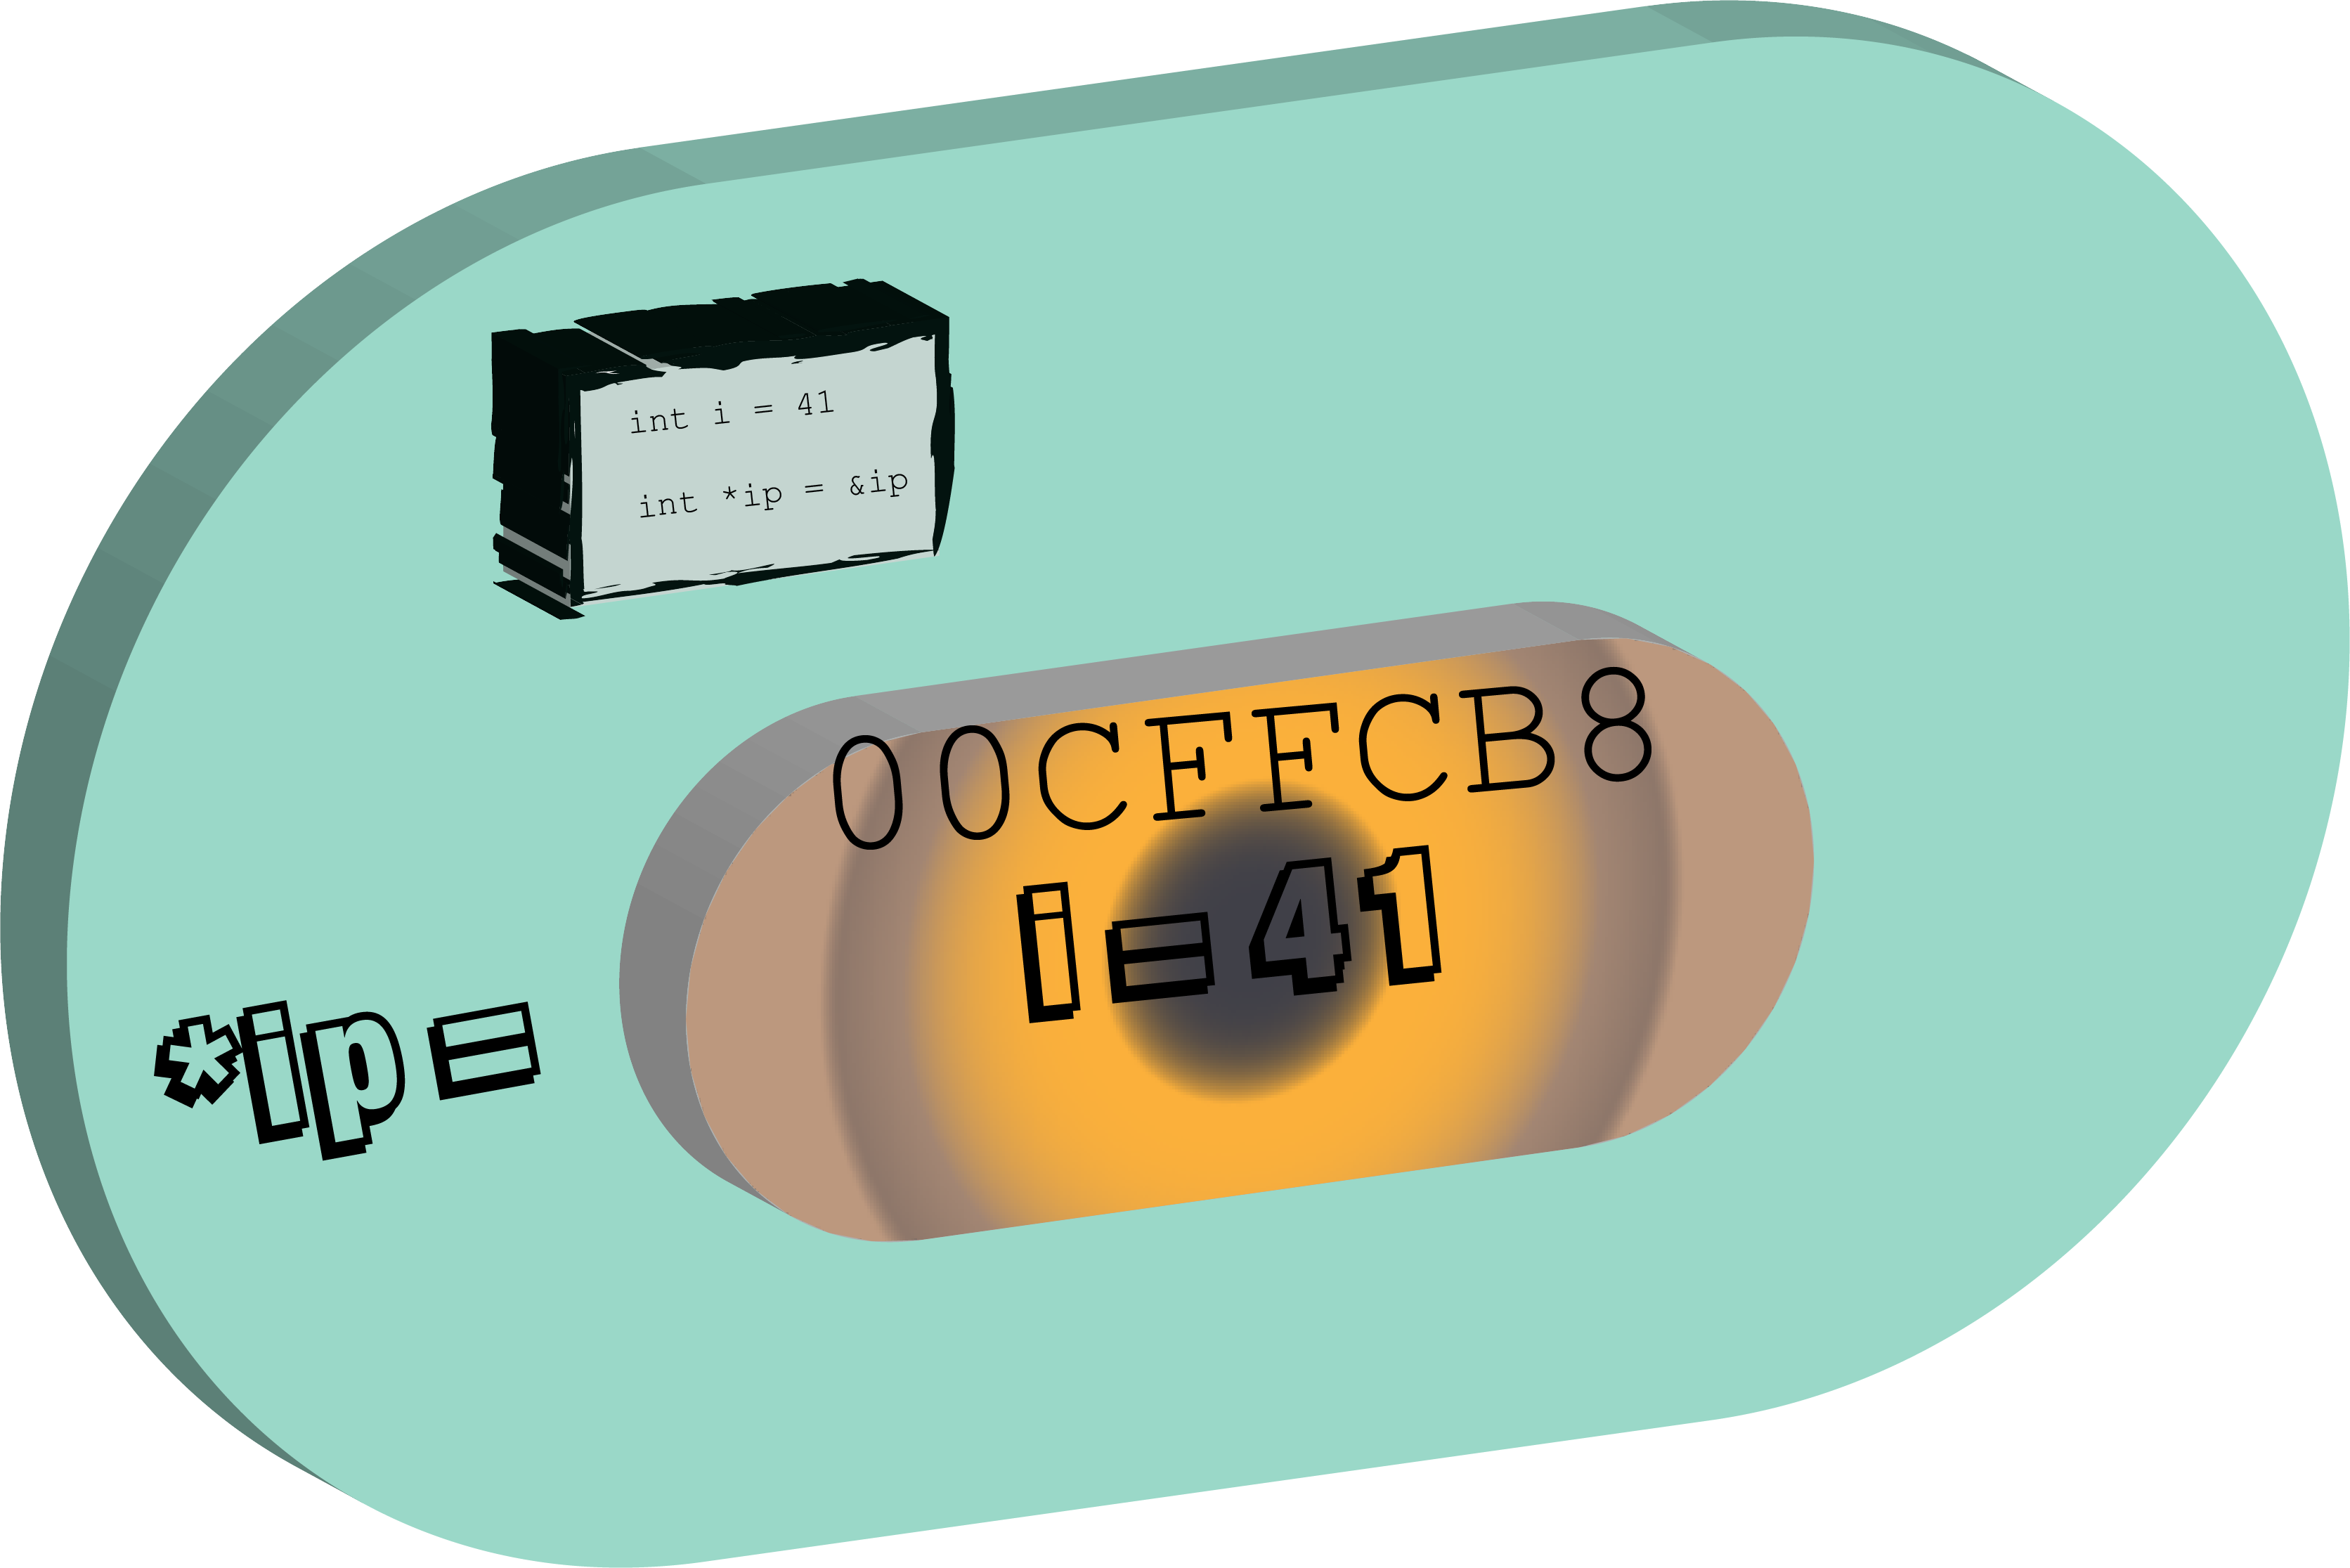
\includegraphics[scale=0.5]{MemoryAddress}
	 	\caption{آدرس حافظه و دیرفرنس کردن}
	 \end{figure}
	 
	 به \lr{\mono\lstinline|&i|} \textbf{اشاره ی مرجعی}\footnote{Reference} به i میگوییم. کلا برای اشاره مرجعی به هر متغیری، از علامت امپرسند استفاده میکنیم. ذر بخشهای بعد، مصرف آنرا خواهید دید.
	 
	 \subsection{توابع در \lr{C++}}\label{cppfunc}
	 
	 توابع در \lr{C++} یک نوع برگشت دارند، و چندین پارامتر با انواع مختلف میپزیرند. تابع main یک تابع int است چون یک عدد صحیح باز میگرداند. توابع در دو مرحله ساخته میشوند، اعلامیه و تعیینیه. اکثر اوقات، اعلامیه در فایلهای سَری انجام میپذیرد و تعیینیه در فایلهای سورس. اما اعلامیه همواره لازم نیست، و میتوان بدون اعلام کردن یک تابع، آن را تعیین کرد.
	 
	 
	 
	 
	 
	 
	 
	 
	 
	 
	 
	 
	 
	 
	 
	 
\end{document}